\documentclass[11pt,a4paper,oneside]{report}
\usepackage{amsmath,amssymb,calc,ifthen}
\usepackage{float}
%\usepackage{cancel}
\usepackage[table,usenames,dvipsnames]{xcolor} % for coloured cells in tables
\usepackage{tikz}
% Allows us to click on links and references!
\usepackage{hyperref}
\usepackage{url}
\hypersetup{
colorlinks,
citecolor=black,
filecolor=black,
linkcolor=black,
urlcolor=black
}
% Nice package for plotting graphs
% See excellent guide:
% http://www.tug.org/TUGboat/tb31-1/tb97wright-pgfplots.pdf
\usetikzlibrary{plotmarks,shapes}
\usepackage{amsmath,graphicx}
\usepackage{epstopdf}
\usepackage{caption}
\usepackage{subcaption}
% highlight - useful for TODOs and similar
\usepackage{color}
\newcommand{\hilight}[1]{\colorbox{yellow}{#1}}
\newcommand\ci{\perp\!\!\!\perp} % perpendicular sign
\newcommand*\rfrac[2]{{}^{#1}\!/_{#2}} % diagonal fraction
\newcommand\SLASH{\char`\\}
\usepackage{listings}
% margin size
\usepackage[margin=0.65in]{geometry}

\usepackage{titlesec} % reduce spacing after subsections

\titlespacing\subsection{0pt}{4pt plus 4pt minus 2pt}{4pt plus 2pt minus 2pt}

\usepackage{multicol}

\tikzstyle{state}=[circle,thick,draw=black, align=center, minimum size=2.1cm,
inner sep=0]
\tikzstyle{vertex}=[circle,thick,draw=black]
\tikzstyle{terminal}=[rectangle,thick,draw=black]
\tikzstyle{edge} = [draw,thick]
\tikzstyle{lo} = [edge,dotted]
\tikzstyle{hi} = [edge]
\tikzstyle{trans} = [edge,->]
\definecolor{mygreen}{rgb}{0,0.6,0}
\definecolor{mygray}{rgb}{0.5,0.5,0.5}
\definecolor{mymauve}{rgb}{0.58,0,0.82}
\DeclareMathOperator*{\argmin}{arg\,min}
\DeclareMathOperator*{\argmax}{arg\,max}
\lstset{ %
backgroundcolor=\color{white}, % choose the background color; you must add
%\usepackage{color} or \usepackage{xcolor}
basicstyle=\footnotesize, % the size of the fonts that are used for the
%code
breakatwhitespace=false, % sets if automatic breaks should only happen
%at whitespace
breaklines=true, % sets automatic line breaking
captionpos=b, % sets the caption-position to bottom
commentstyle=\color{mygreen}, % comment style
deletekeywords={...}, % if you want to delete keywords from the
%given language
escapeinside={\%*}{*)}, % if you want to add LaTeX within your code
extendedchars=true, % lets you use non-ASCII characters; for
%8-bits encodings only, does not work with UTF-8
frame=single, % adds a frame around the code
keepspaces=true, % keeps spaces in text, useful for keeping
%indentation of code (possibly needs columns=flexible)
keywordstyle=\color{blue}, % keyword style
language=Octave, % the language of the code
morekeywords={*,...}, % if you want to add more keywords to the set
numbers=left, % where to put the line-numbers; possible
%values are (none, left, right)
numbersep=5pt, % how far the line-numbers are from the code
numberstyle=\tiny\color{mygray}, % the style that is used for the line-numbers
rulecolor=\color{black}, % if not set, the frame-color may be changed
%on line-breaks within not-black text (e.g. comments (green here))
showspaces=false, % show spaces everywhere adding particular
%underscores; it overrides 'showstringspaces'
showstringspaces=false, % underline spaces within strings only
showtabs=false, % show tabs within strings adding particular
%underscores
stepnumber=2, % the step between two line-numbers. If it's
%1, each line will be numbered
stringstyle=\color{mymauve}, % string literal style
tabsize=2, % sets default tabsize to 2 spaces
title=\lstname % show the filename of files included with
%\lstinputlisting; also try caption instead of title
}
\title{Computational Modelling for Biomedical Imaging - Individual Report}
\author{
Razvan Valentin Marinescu\\
Student Number: 14060166\\
\texttt{razvan.marinescu.14@ucl.ac.uk}
}



\begin{document}
\belowdisplayskip=12pt plus 3pt minus 9pt
\belowdisplayshortskip=7pt plus 3pt minus 4pt

\begin{titlepage}
\begin{center}

% Upper part of the page. The '~' is needed because \\
% only works if a paragraph has started.

\includegraphics[width=0.2\textwidth]{ucl-logo2}~\\[1cm]

\textsc{\LARGE University College London}\\[1.5cm]

\newcommand{\HRule}{\rule{\linewidth}{0.5mm}}

% Title
\HRule \\[0.4cm]
{ \Large Computational Modelling for Biomedical Imaging - Individual Report \\[0.4cm] }

\HRule \\[1.5cm]

% Author and supervisor
\begin{minipage}{0.4\textwidth}
% \begin{flushleft} \large
\centering
\emph{Author:}\\
R\u{a}zvan Valentin \textsc{Marinescu}\\
\href{razvan.marinescu.14@ucl.ac.uk}{razvan.marinescu.14@ucl.ac.uk}\\
% \end{flushleft}
\end{minipage}


\vfill

\vfill
\vfill

EPSRC Centre for Doctoral Training in Medical Imaging\\ University College London

\vfill

% Bottom of the page
{\large \today}

\end{center}
\end{titlepage}


%\maketitle{}



\rowcolors{2}{gray!25}{white}

\subsection*{Task 1 - Registration assessment}

\begin{figure}[H]
  \centering
  \begin{subfigure}[b]{0.1\textwidth}
    Reg 1\\\\\\\\
  \end{subfigure}%
  \hspace*{-1.9em}
  \begin{subfigure}[b]{0.3\textwidth}
	  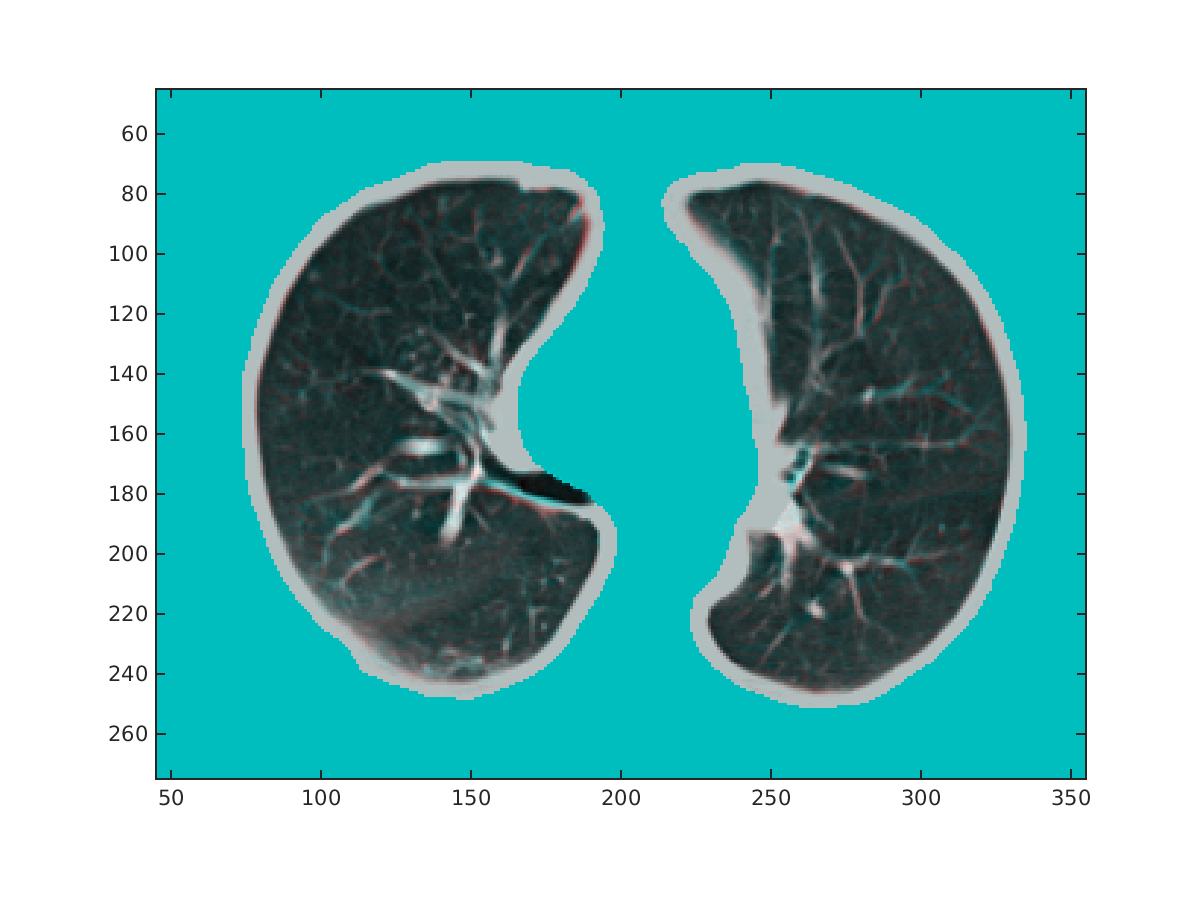
\includegraphics[width=\textwidth, trim=20 20 20 20]{figures/reg1/reg1_1_66.png}
  \end{subfigure}%
%         ~ %add desired spacing between images, e. g. ~, \quad, \qquad, \hfill etc.
    %(or a blank line to force the subfigure onto a new line)
  \begin{subfigure}[b]{0.3\textwidth}
	  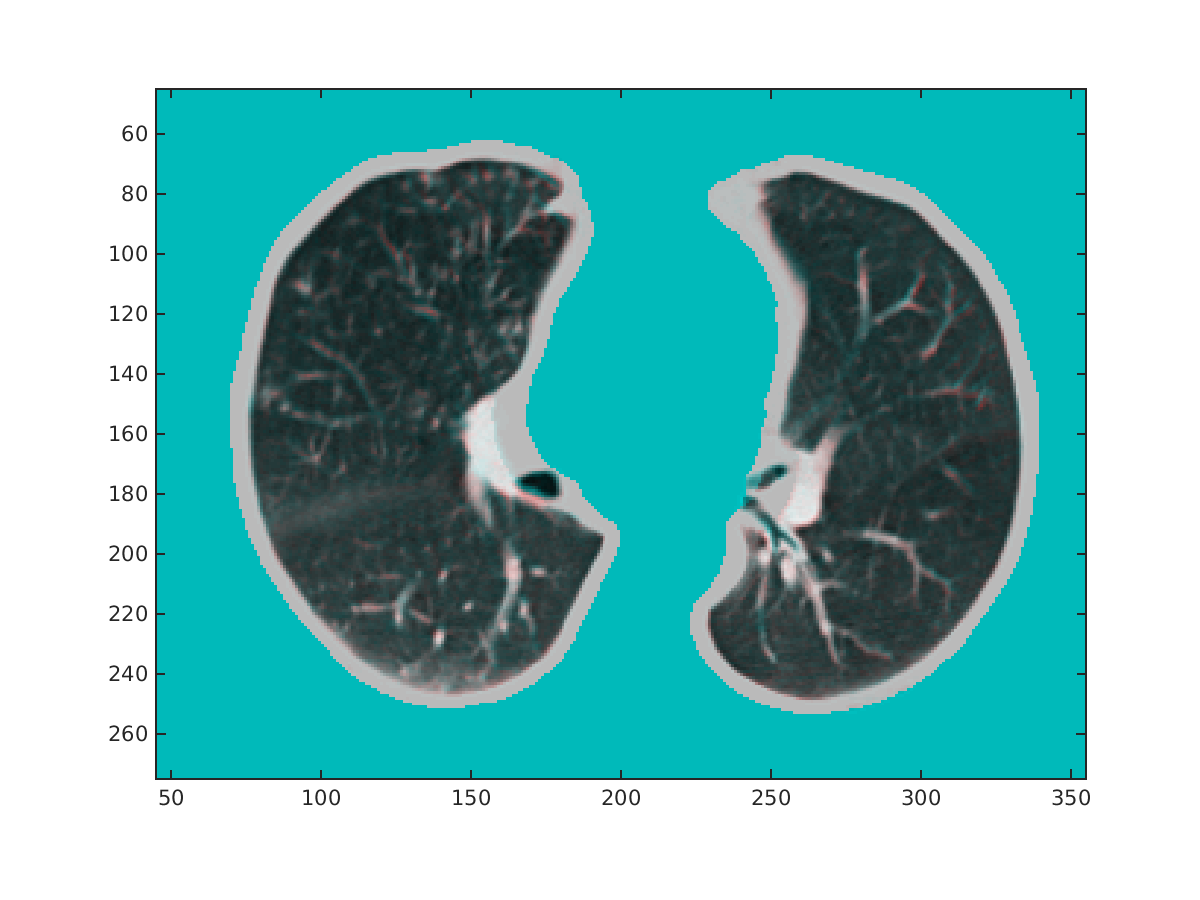
\includegraphics[width=\textwidth, trim=20 20 20 20]{figures/reg1/reg2_5_60.png}
  \end{subfigure}
%         ~ %add desired spacing between images, e. g. ~, \quad, \qquad, \hfill etc.
    %(or a blank line to force the subfigure onto a new line)
  \begin{subfigure}[b]{0.3\textwidth}
	  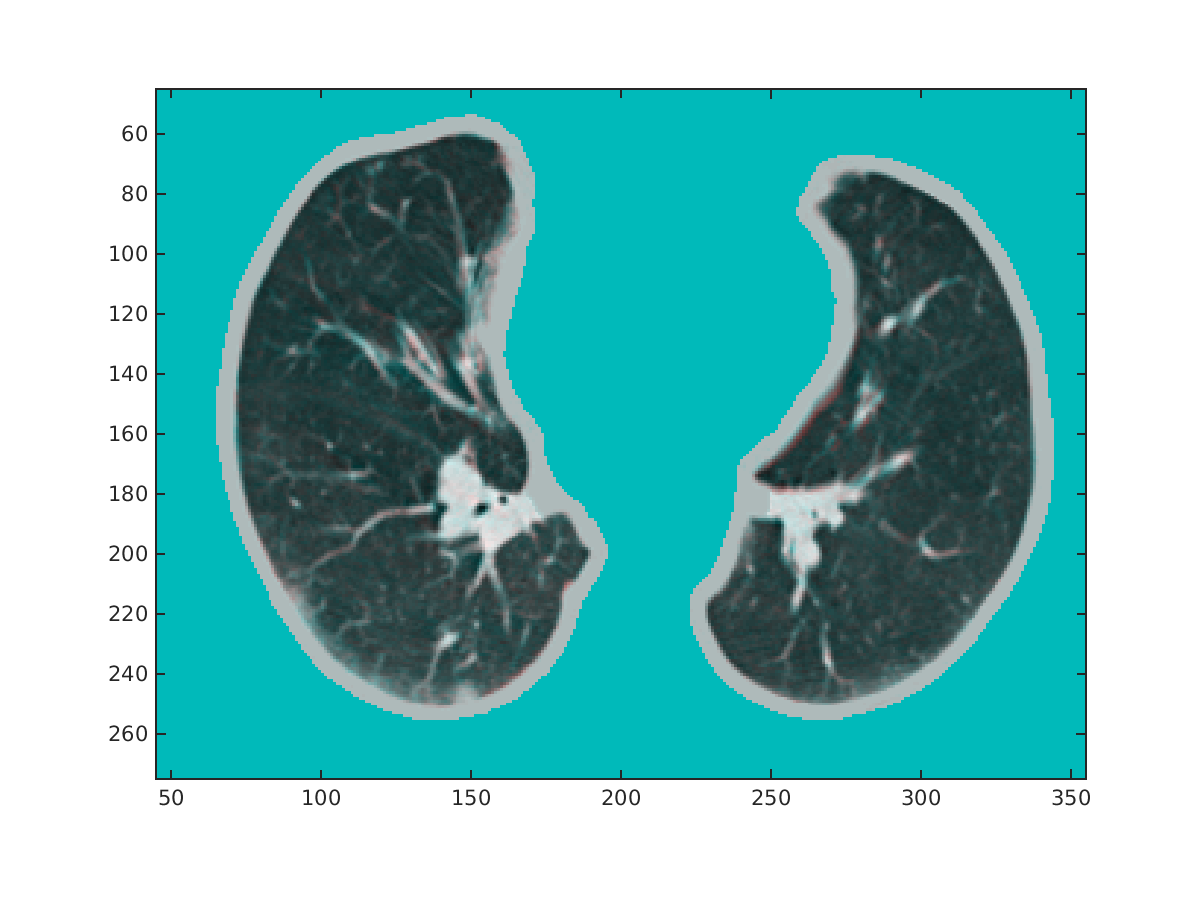
\includegraphics[width=\textwidth, trim=20 20 20 20]{figures/reg1/reg3_2_49.png}
  \end{subfigure}
  
%         ~

  \begin{subfigure}[b]{0.1\textwidth}
    Reg 2\\\\\\\\\\
  \end{subfigure}%
  \hspace*{-1.9em}
  \begin{subfigure}[b]{0.3\textwidth}
	  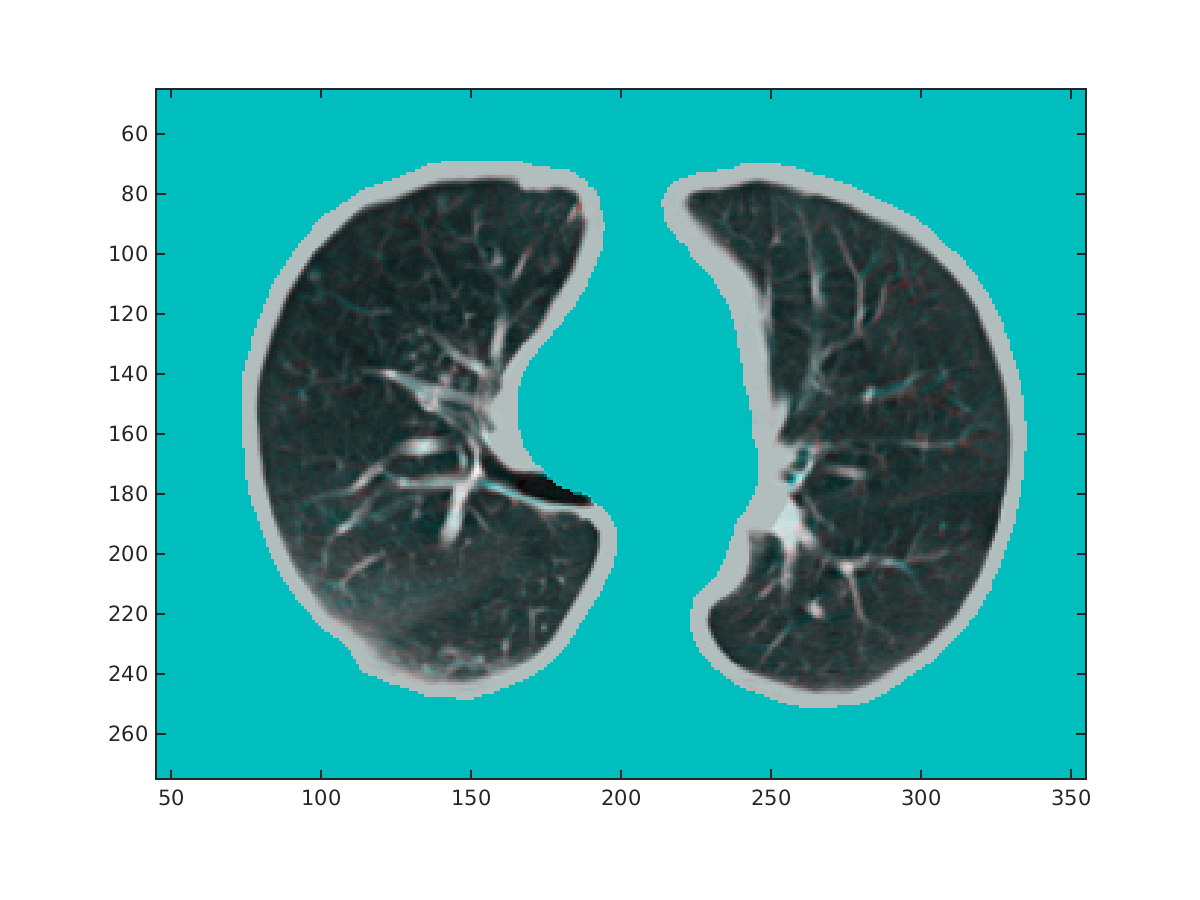
\includegraphics[width=\textwidth, trim=20 20 20 20]{figures/reg2/reg1_1_66.png}
	  \caption{Couch 1, volume 1, slice 66}
	  \label{fig:c11}
  \end{subfigure}%
%         ~ %add desired spacing between images, e. g. ~, \quad, \qquad, \hfill etc.
%           %(or a blank line to force the subfigure onto a new line)
  \begin{subfigure}[b]{0.3\textwidth}
	  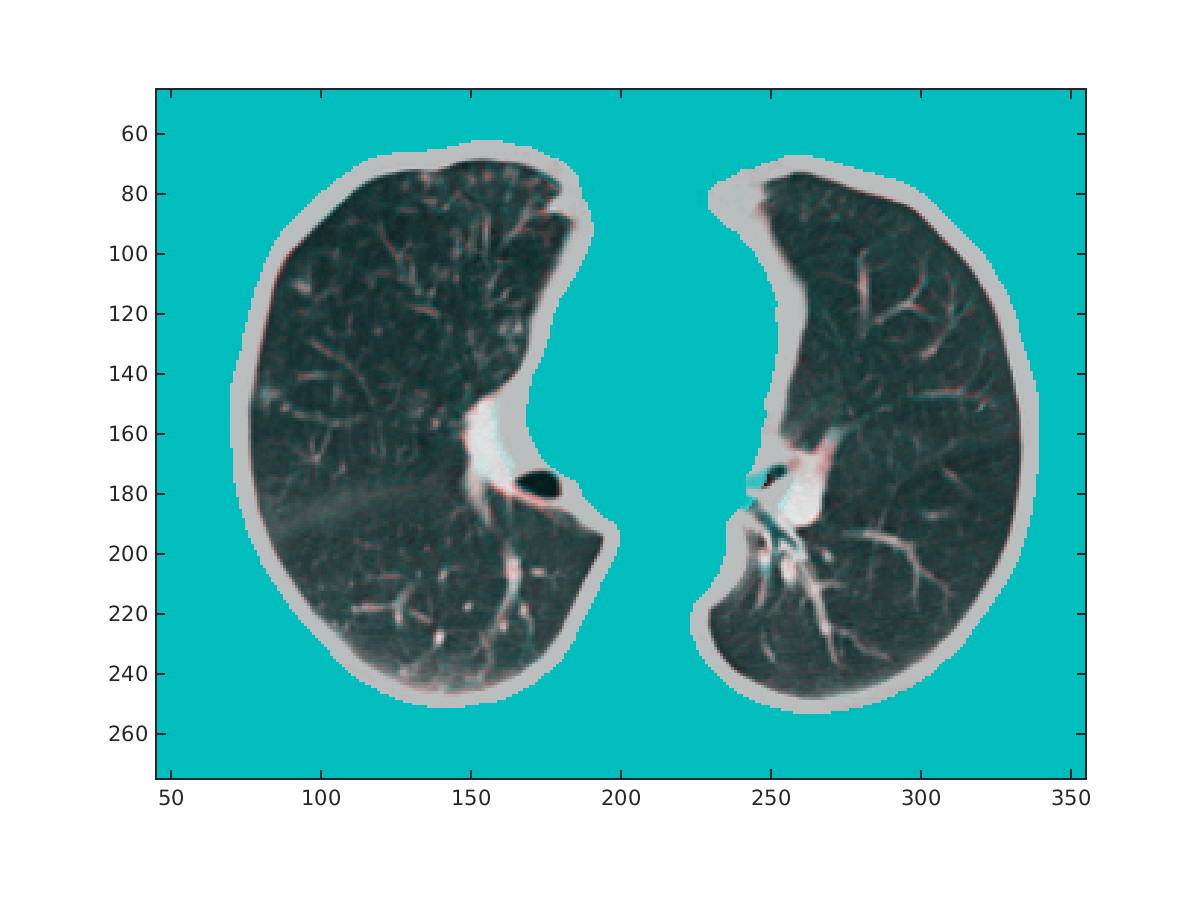
\includegraphics[width=\textwidth, trim=20 20 20 20]{figures/reg2/reg2_5_60.png}
	  \caption{Couch 2, volume 5, slice 60}
	  \label{fig:c12}
  \end{subfigure}
%         ~ %add desired spacing between images, e. g. ~, \quad, \qquad, \hfill etc.
    %(or a blank line to force the subfigure onto a new line)
  \begin{subfigure}[b]{0.3\textwidth}
	  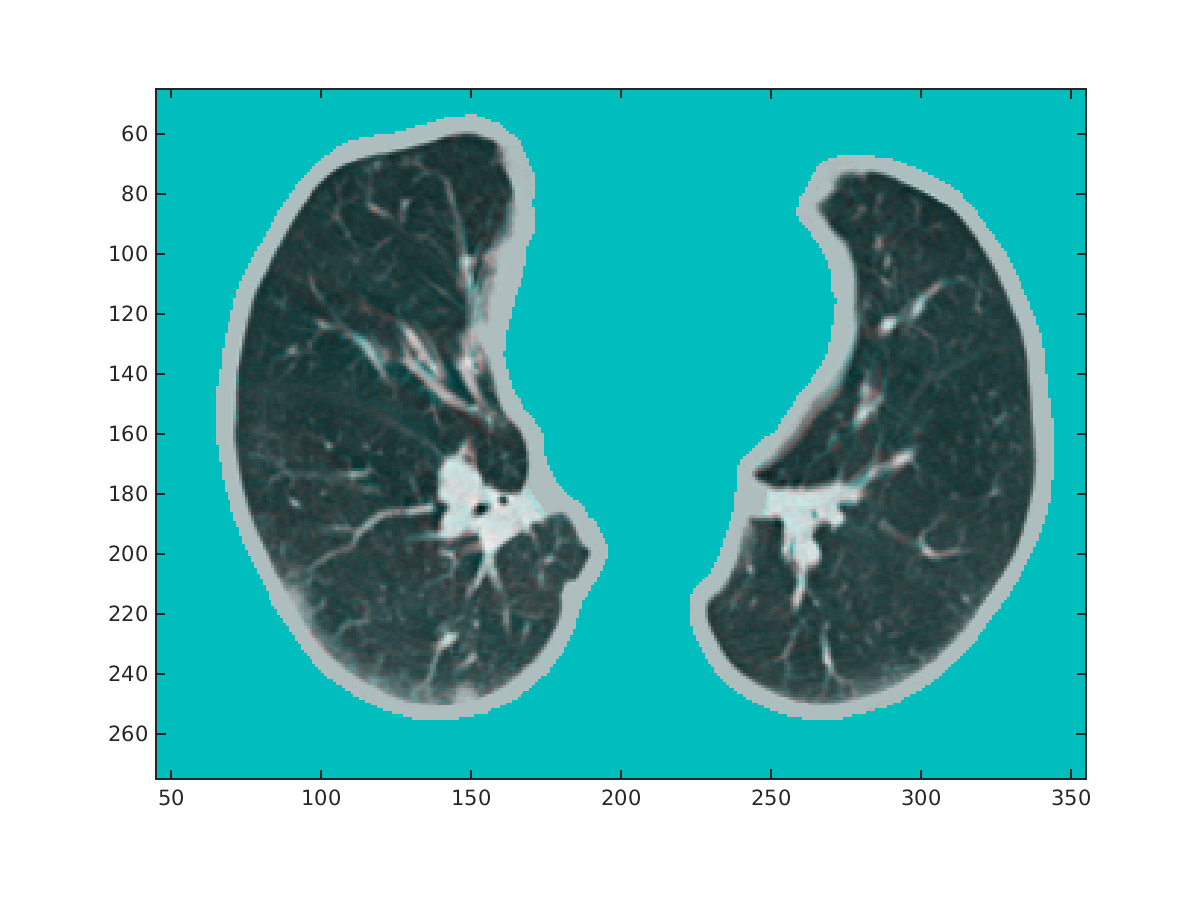
\includegraphics[width=\textwidth, trim=20 20 20 20]{figures/reg2/reg3_2_49.png}
	  \caption{Couch 3, volume 2, slice 49}
	  \label{fig:c13}
  \end{subfigure}
  
  ~
  \vfill
  
  \begin{subfigure}[b]{0.1\textwidth}
    Reg 1\\\\\\\\
  \end{subfigure}%
  \hspace*{-1.9em}
  \begin{subfigure}[b]{0.3\textwidth}
	  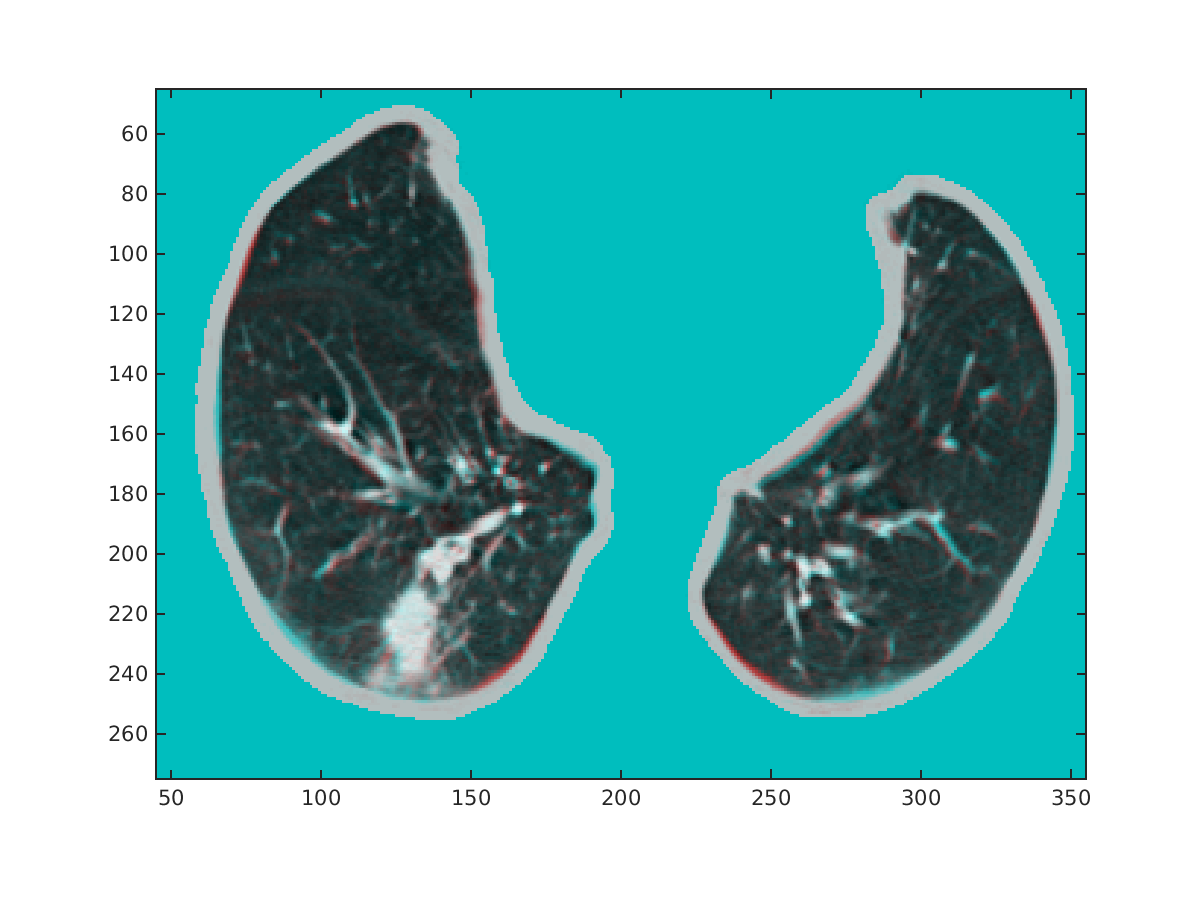
\includegraphics[width=\textwidth, trim=20 20 20 20]{figures/reg1/reg4_8_37.png}
  \end{subfigure}%
%         ~ %add desired spacing between images, e. g. ~, \quad, \qquad, \hfill etc.
    %(or a blank line to force the subfigure onto a new line)
  \begin{subfigure}[b]{0.3\textwidth}
	  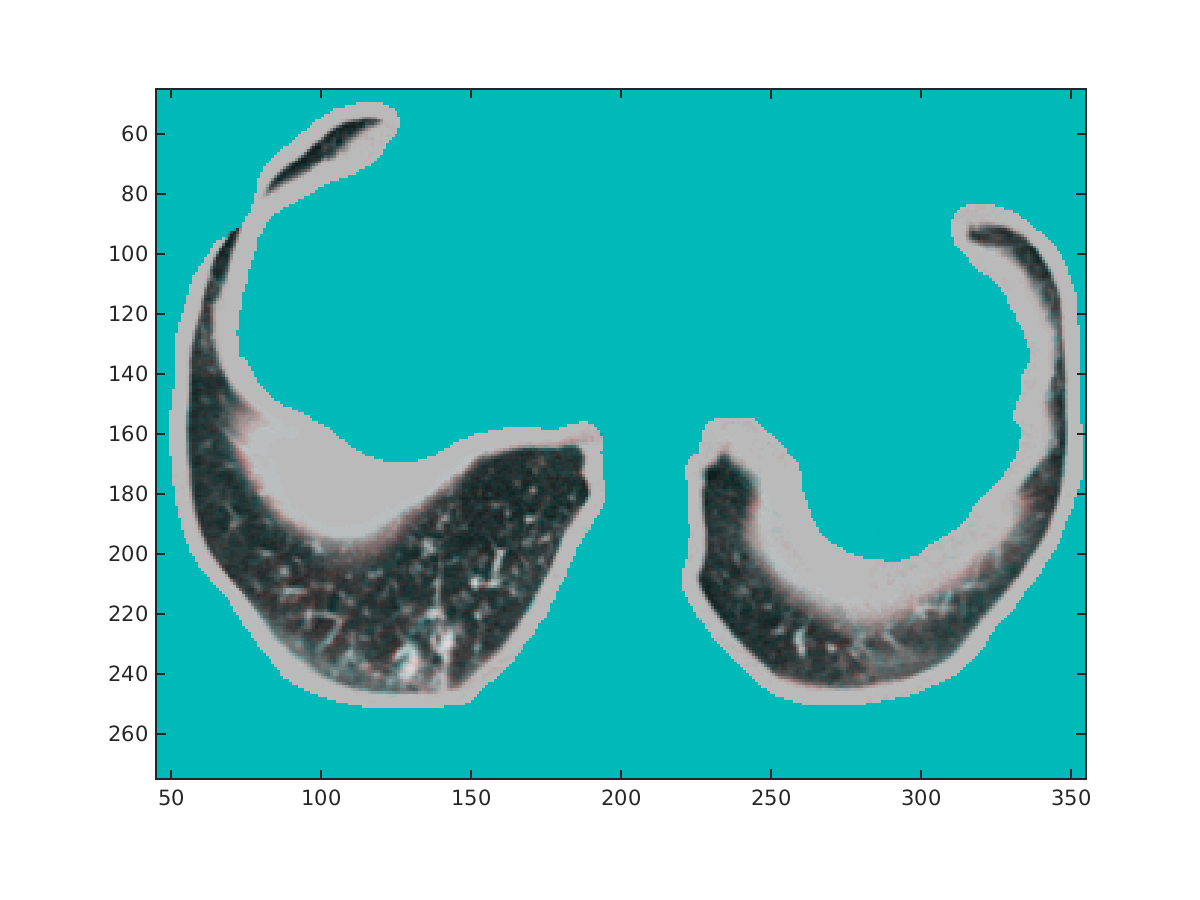
\includegraphics[width=\textwidth, trim=20 20 20 20]{figures/reg1/reg5_4_25.png}
  \end{subfigure}
%         ~ %add desired spacing between images, e. g. ~, \quad, \qquad, \hfill etc.
    %(or a blank line to force the subfigure onto a new line)
  \begin{subfigure}[b]{0.3\textwidth}
	  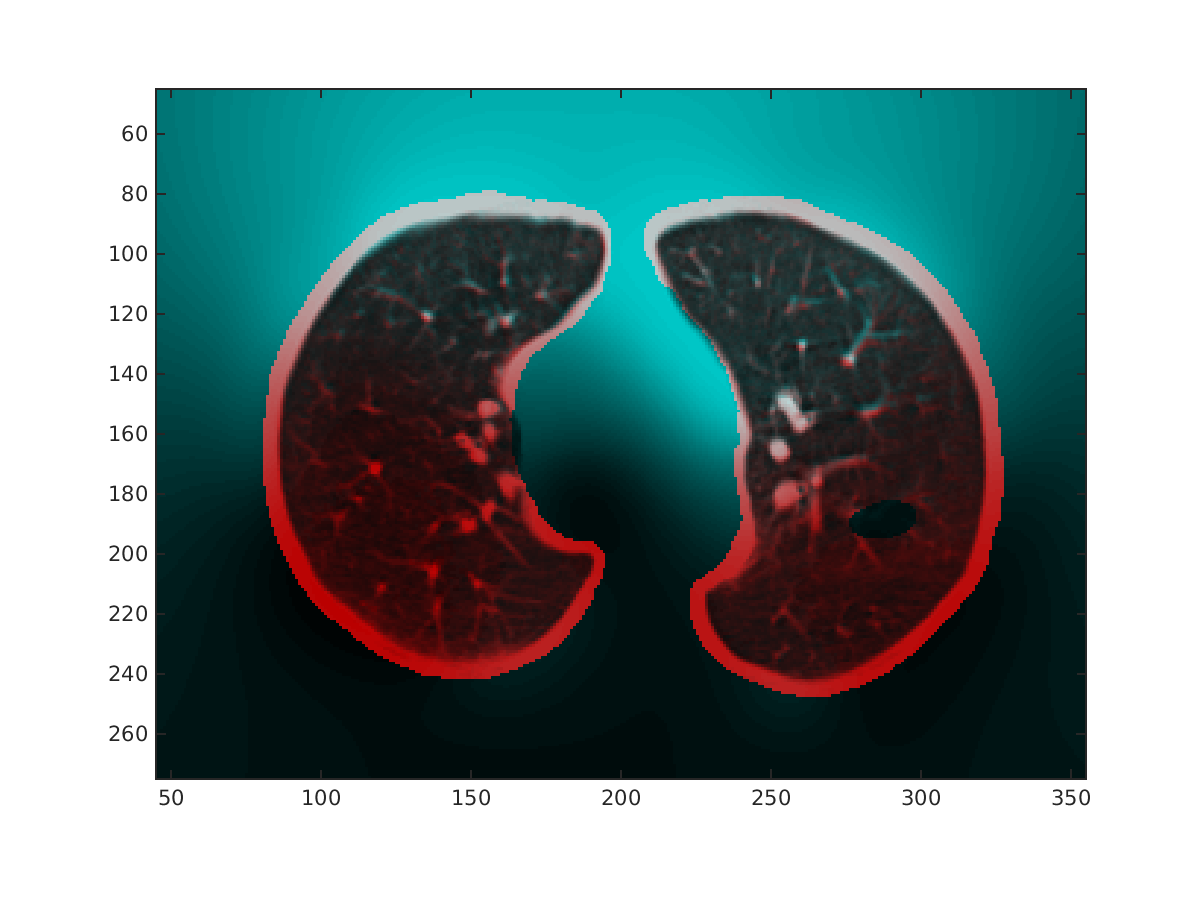
\includegraphics[width=\textwidth, trim=20 20 20 20]{figures/reg1/reg1_6_76.png}
  \end{subfigure}
  
%         ~

  \begin{subfigure}[b]{0.1\textwidth}
    Reg 2\\\\\\\\\\
  \end{subfigure}%
  \hspace*{-1.9em}
  \begin{subfigure}[b]{0.3\textwidth}
	  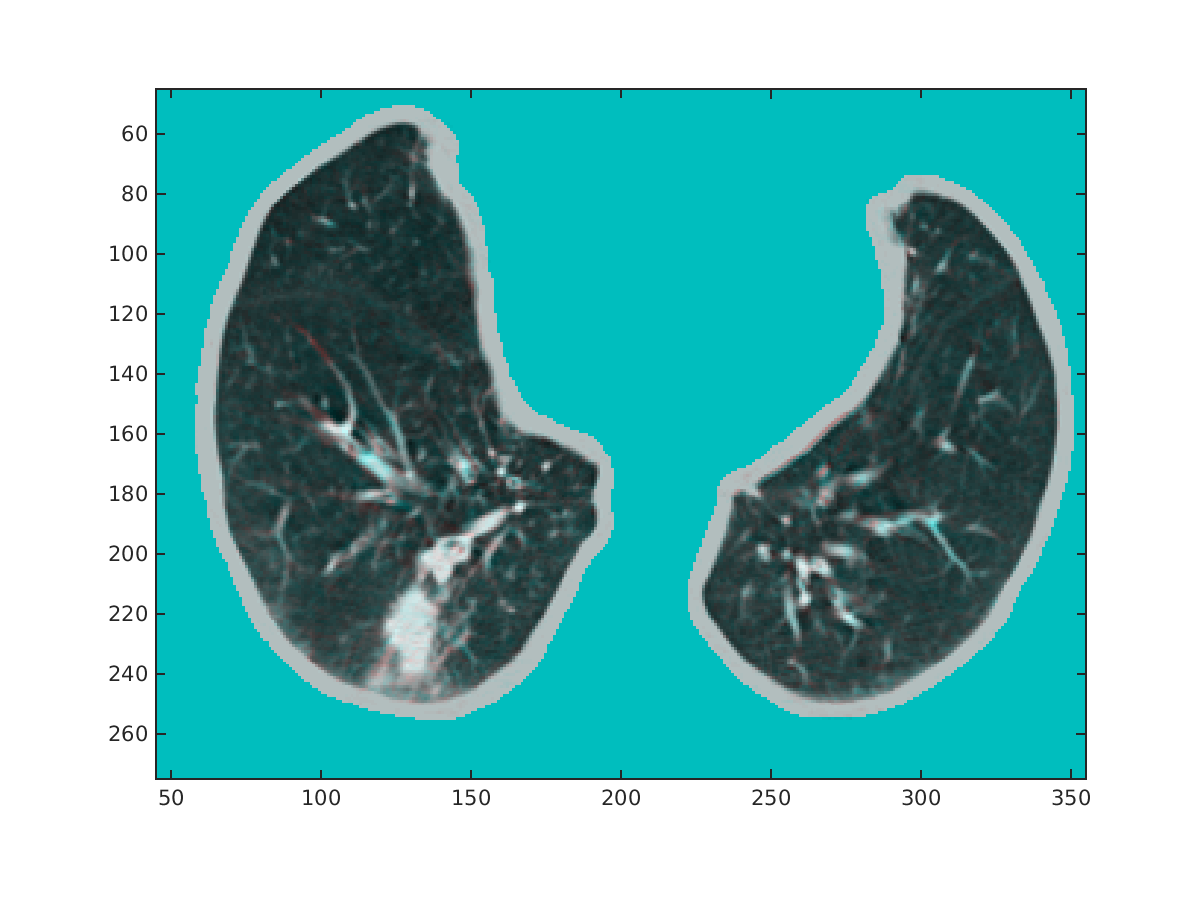
\includegraphics[width=\textwidth, trim=20 20 20 20]{figures/reg2/reg4_8_37.png}
	  \caption{Couch 4, volume 8, slice 37}
	  \label{fig:c21}
  \end{subfigure}%
%         ~ %add desired spacing between images, e. g. ~, \quad, \qquad, \hfill etc.
    %(or a blank line to force the subfigure onto a new line)
  \begin{subfigure}[b]{0.3\textwidth}
	  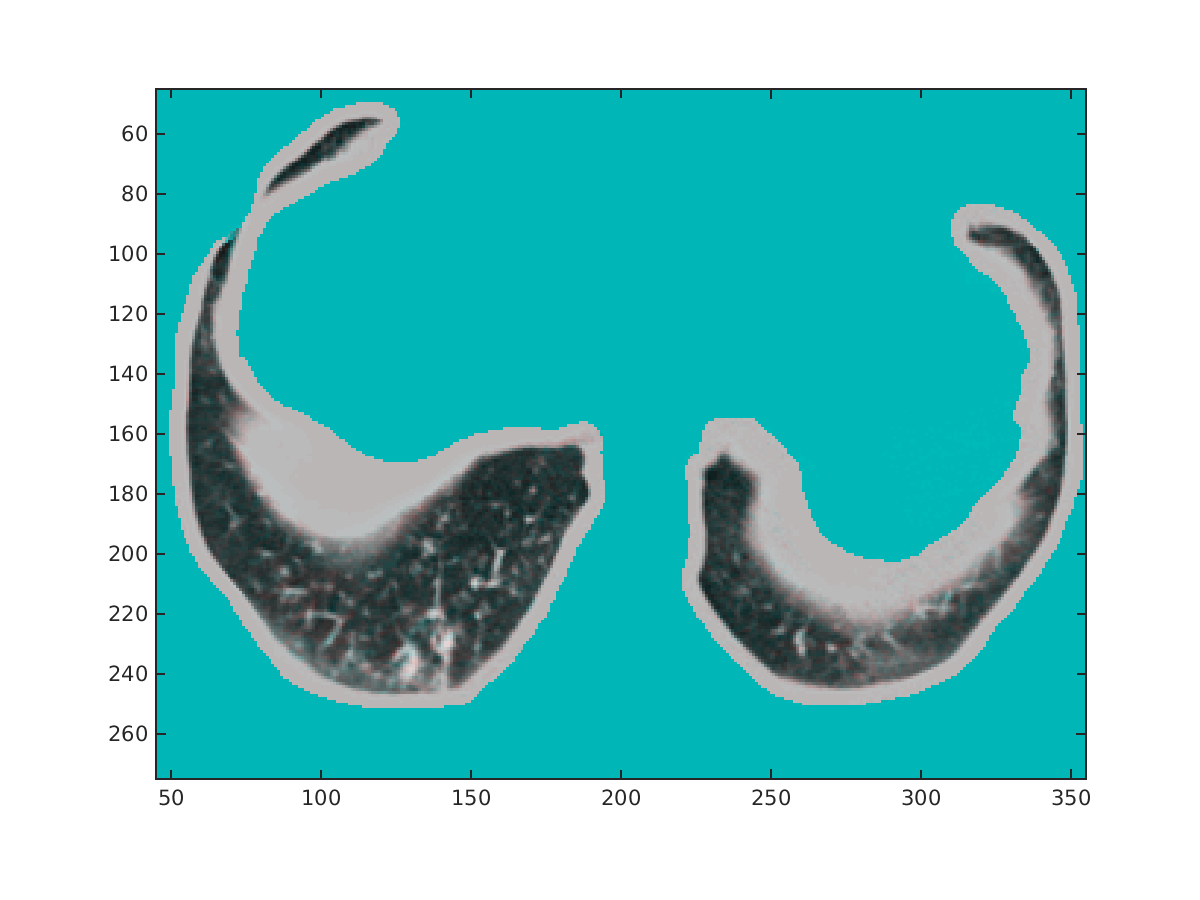
\includegraphics[width=\textwidth, trim=20 20 20 20]{figures/reg2/reg5_4_25.png}
	  \caption{Couch 5, volume 4, slice 25}
	  \label{fig:c22}
  \end{subfigure}
%         ~ %add desired spacing between images, e. g. ~, \quad, \qquad, \hfill etc.
    %(or a blank line to force the subfigure onto a new line)
  \begin{subfigure}[b]{0.3\textwidth}
	  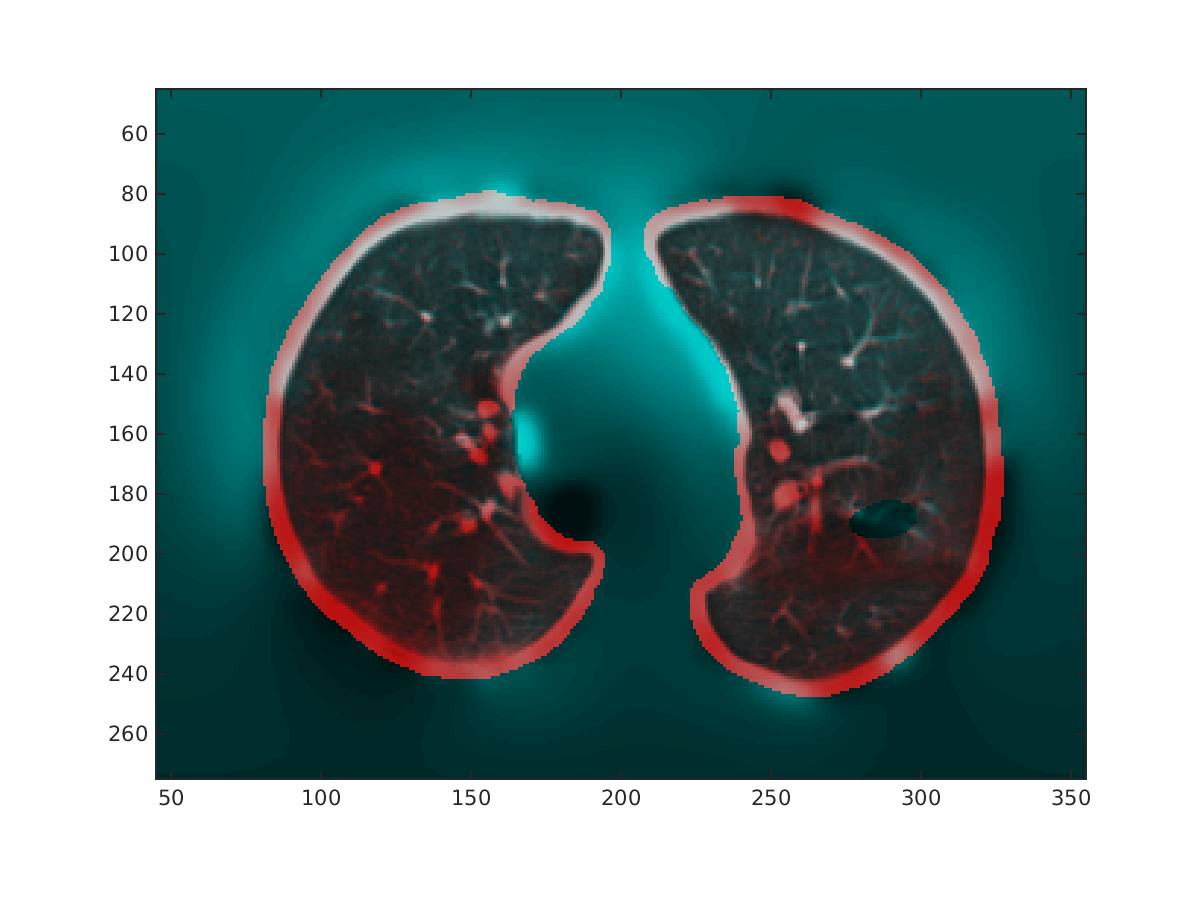
\includegraphics[width=\textwidth, trim=20 20 20 20]{figures/reg2/reg1_6_76.png}
	  \caption{Couch 1, volume 6, slice 76}
	  \label{fig:c23}
  \end{subfigure}
  \caption{Registration results at several different slices and volumes for each couch position. For each subfigure, registration 1 and 2 are shown in the upper and lower figures respectively.}
  \label{fig:c1vis}
\end{figure}


Figure \ref{fig:c1vis} shows the registration results for a few representative slices and volumes over all couch positions. Both registrations perform equally well subfigures (\ref{fig:c11} - \ref{fig:c22}), but yielded a bad registration in subfigure \ref{fig:c23}. Similar bad registrations have been observed in the last slice of each volume. The images show us that there is a considerable ammount of respiratory motion across different slices which needs to be modelled. The shape of the lung is also dramatically different across different couch positions, reaching a concave shape at couch 5. Nevertheless, the segmentation and registration worked fine even for these slices.

\subsection*{Task 2 \& 3 - Fitting the models}

\begin{figure}[H]
  \centering
  \hspace*{-2em}
  \begin{subfigure}[b]{0.33\textwidth}
    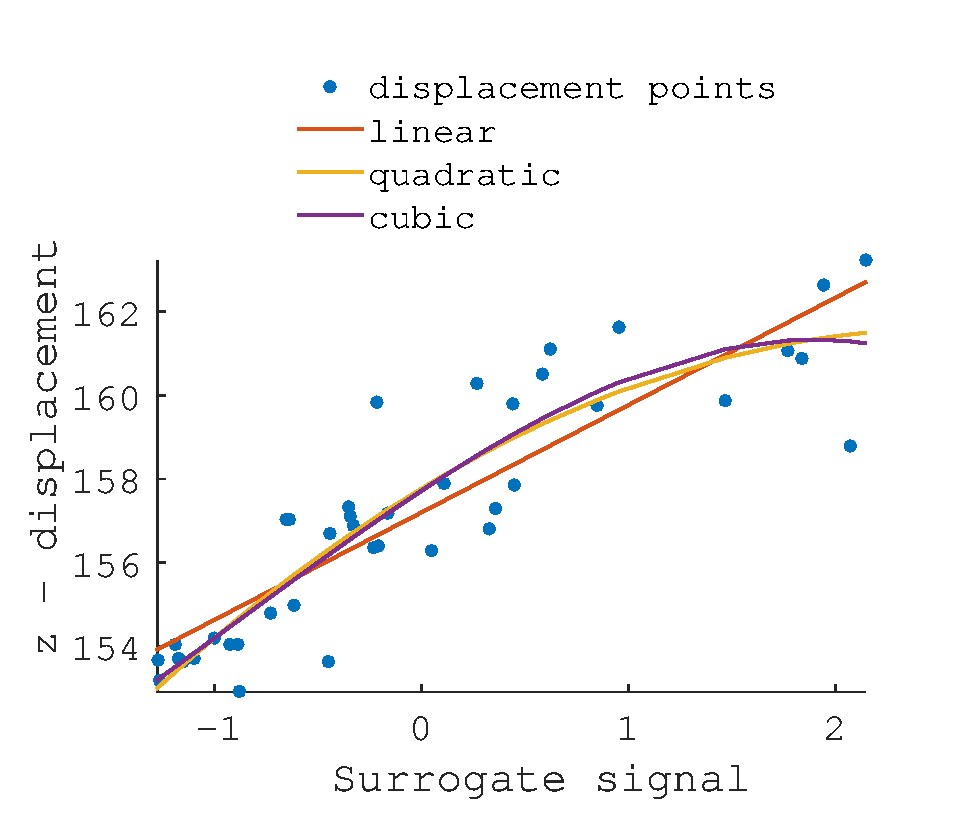
\includegraphics[width=\textwidth]{figures/task2/fit_round1_couch1.eps}
  \end{subfigure}%
    ~ %add desired spacing between images, e. g. ~, \quad, \qquad, \hfill etc.
  %(or a blank line to force the subfigure onto a new line)
  \begin{subfigure}[b]{0.33\textwidth}
    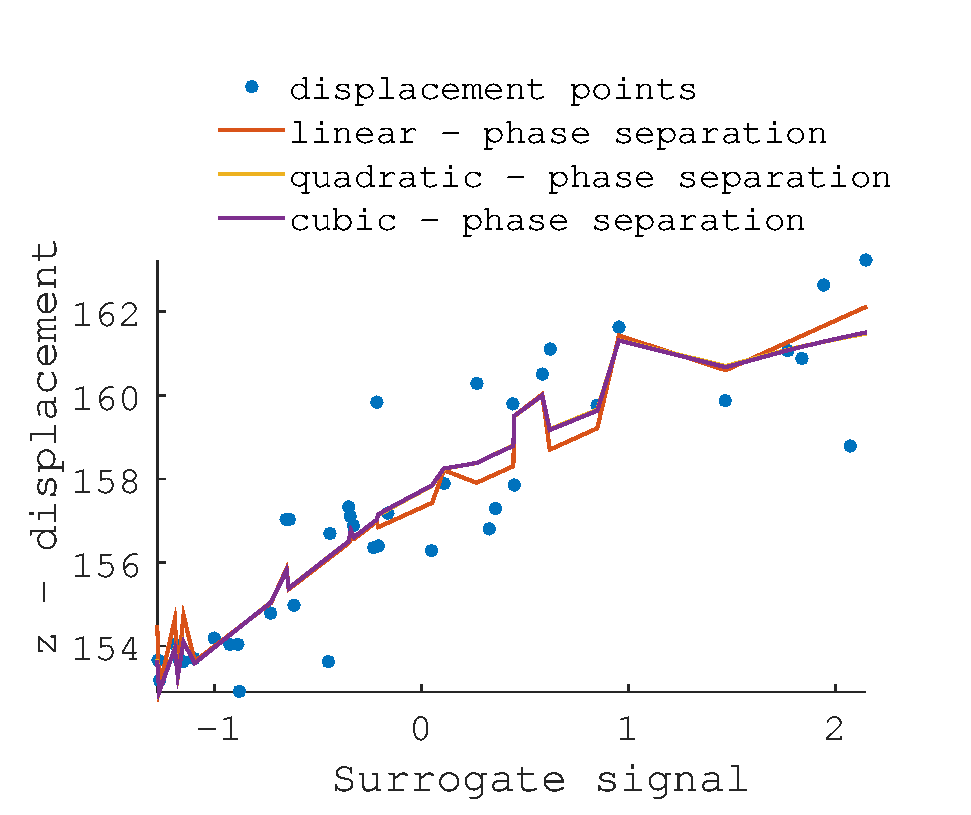
\includegraphics[width=\textwidth]{figures/task2/fit_round2_couch1.eps}
  \end{subfigure}
    ~ %add desired spacing between images, e. g. ~, \quad, \qquad, \hfill etc.
  %     (or a blank line to force the subfigure onto a new line)
  \begin{subfigure}[b]{0.33\textwidth}
    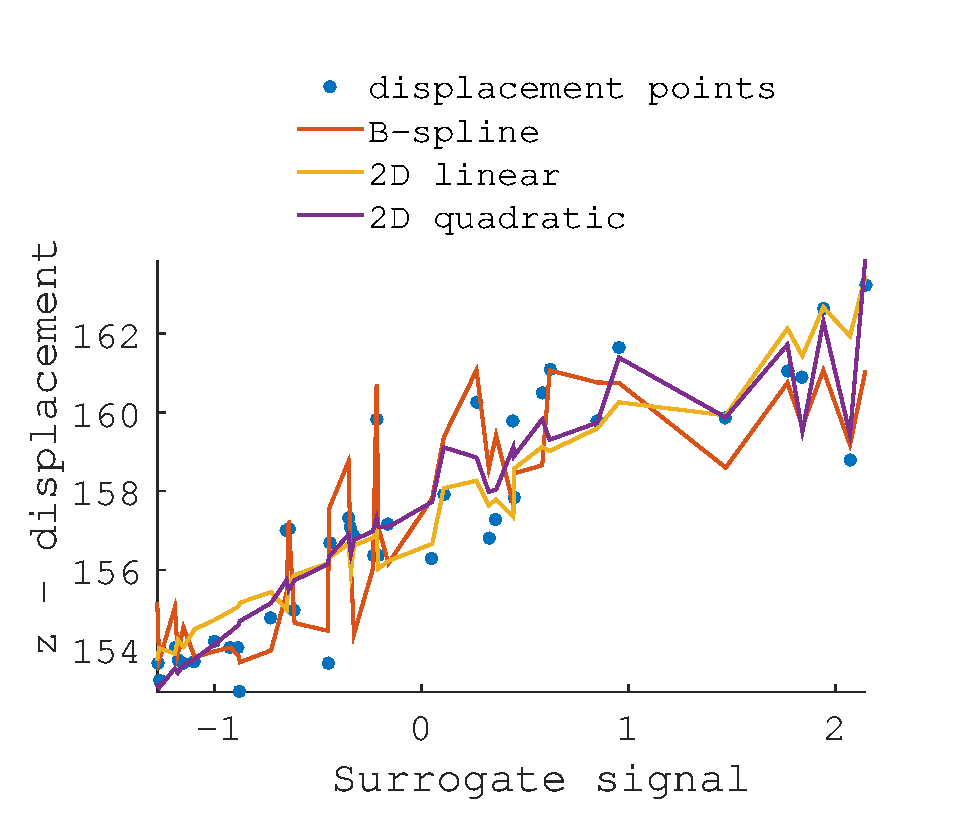
\includegraphics[width=\textwidth]{figures/task2/fit_round3_couch1.eps}
  \end{subfigure}
  (a) Fit for couch position 1, voxel (30,40,33,1,3)
  \vspace*{1em}
  
  \hspace*{-2em}
  \begin{subfigure}[b]{0.33\textwidth}
    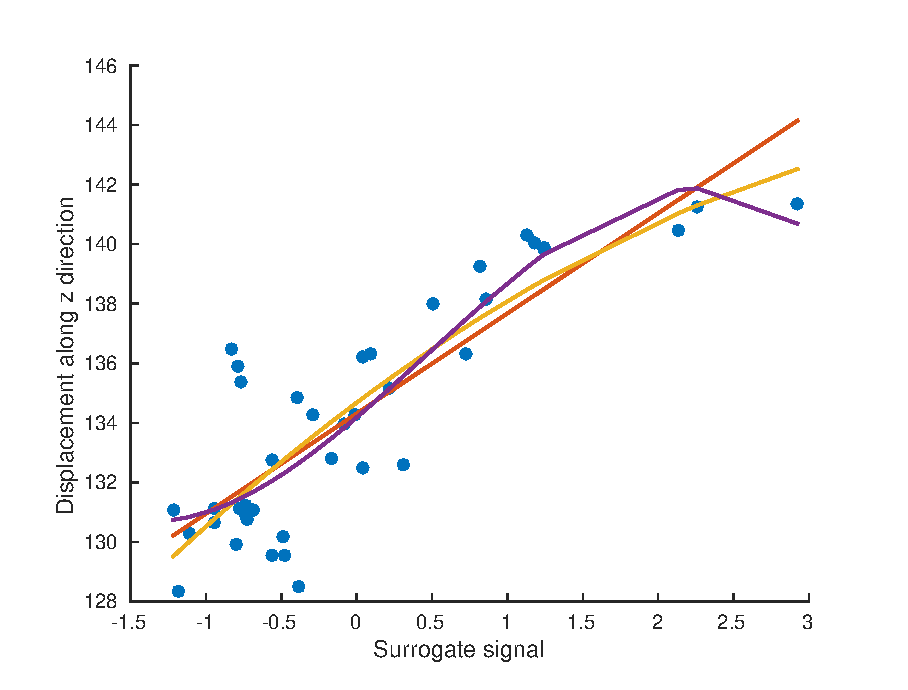
\includegraphics[width=\textwidth, trim=0 0 0 110,clip=true]{figures/task2/fit_round1_couch2.eps}
  \end{subfigure}%
    ~ %add desired spacing between images, e. g. ~, \quad, \qquad, \hfill etc.
%(or a blank line to force the subfigure onto a new line)
  \begin{subfigure}[b]{0.33\textwidth}
    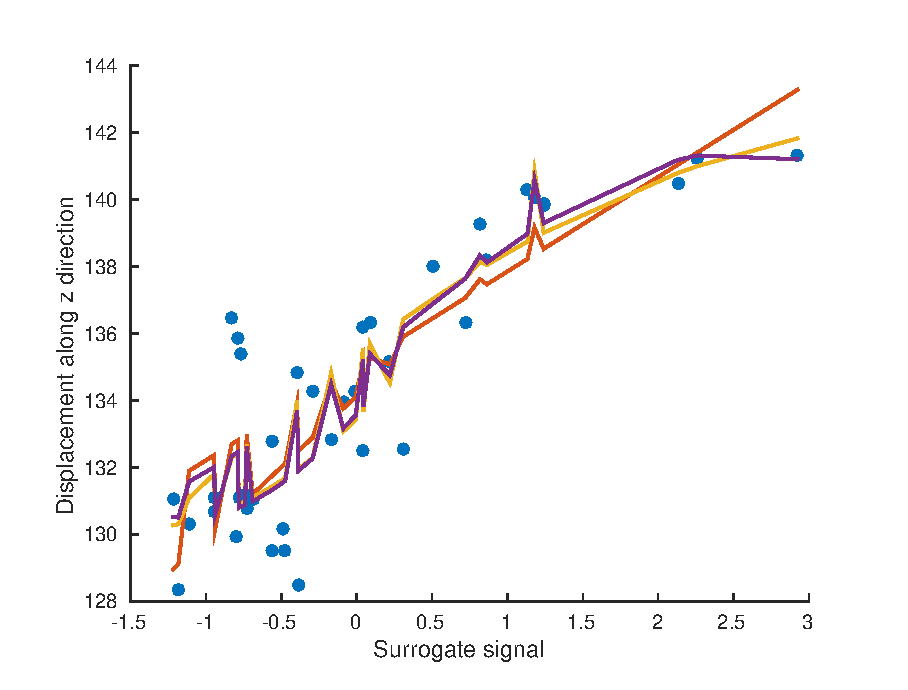
\includegraphics[width=\textwidth, trim=0 0 0 110,clip=true]{figures/task2/fit_round2_couch2.eps}
  \end{subfigure}
    ~ %add desired spacing between images, e. g. ~, \quad, \qquad, \hfill etc.
%     (or a blank line to force the subfigure onto a new line)
  \begin{subfigure}[b]{0.33\textwidth}
    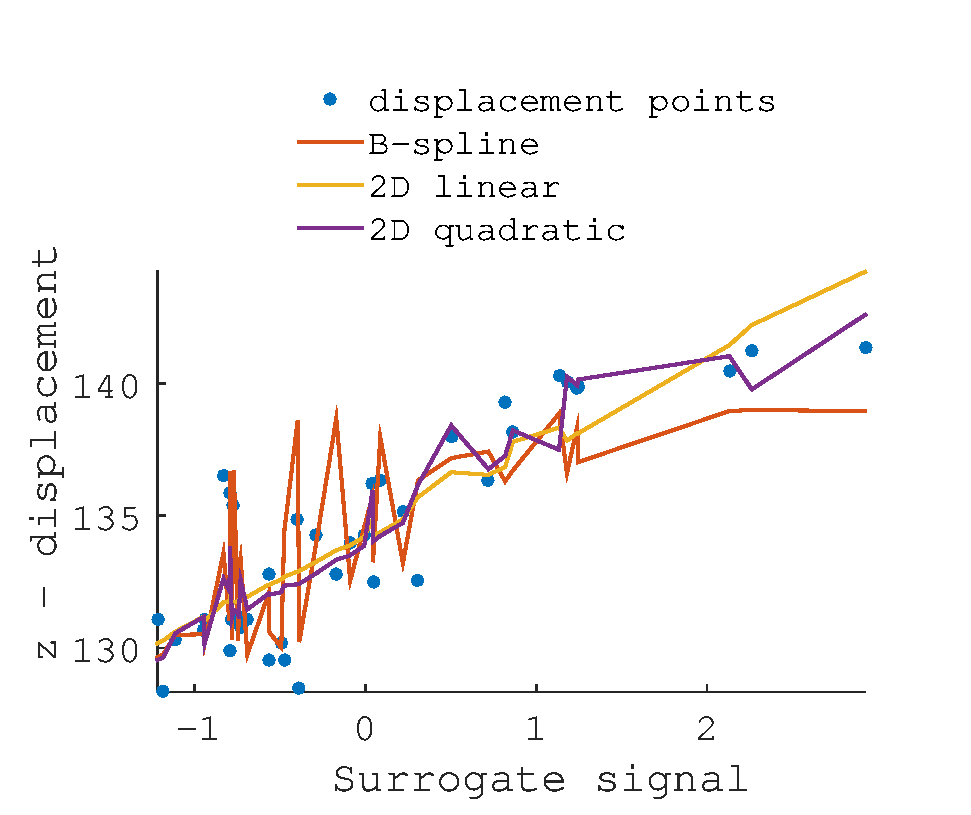
\includegraphics[width=\textwidth, trim=0 0 0 110,clip=true]{figures/task2/fit_round3_couch2.eps}
  \end{subfigure}
  (b) Fit for couch position 2, voxel (30,40,28,1,3)
  \vspace*{1em}
  
    \hspace*{-2em}
  \begin{subfigure}[b]{0.33\textwidth}
    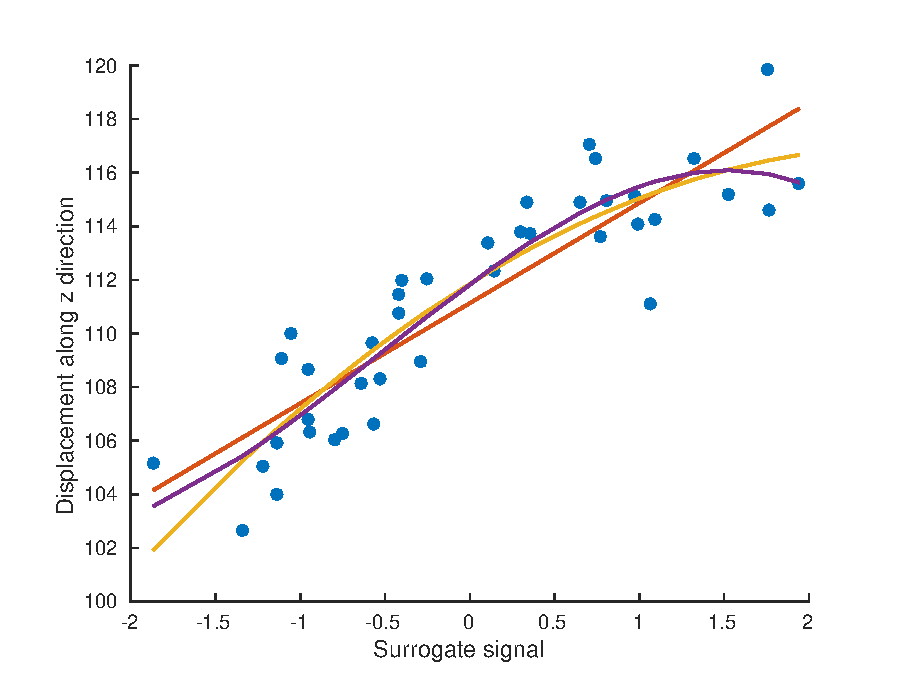
\includegraphics[width=\textwidth, trim=0 0 0 110,clip=true]{figures/task2/fit_round1_couch3.eps}
  \end{subfigure}%
    ~ %add desired spacing between images, e. g. ~, \quad, \qquad, \hfill etc.
%(or a blank line to force the subfigure onto a new line)
  \begin{subfigure}[b]{0.33\textwidth}
    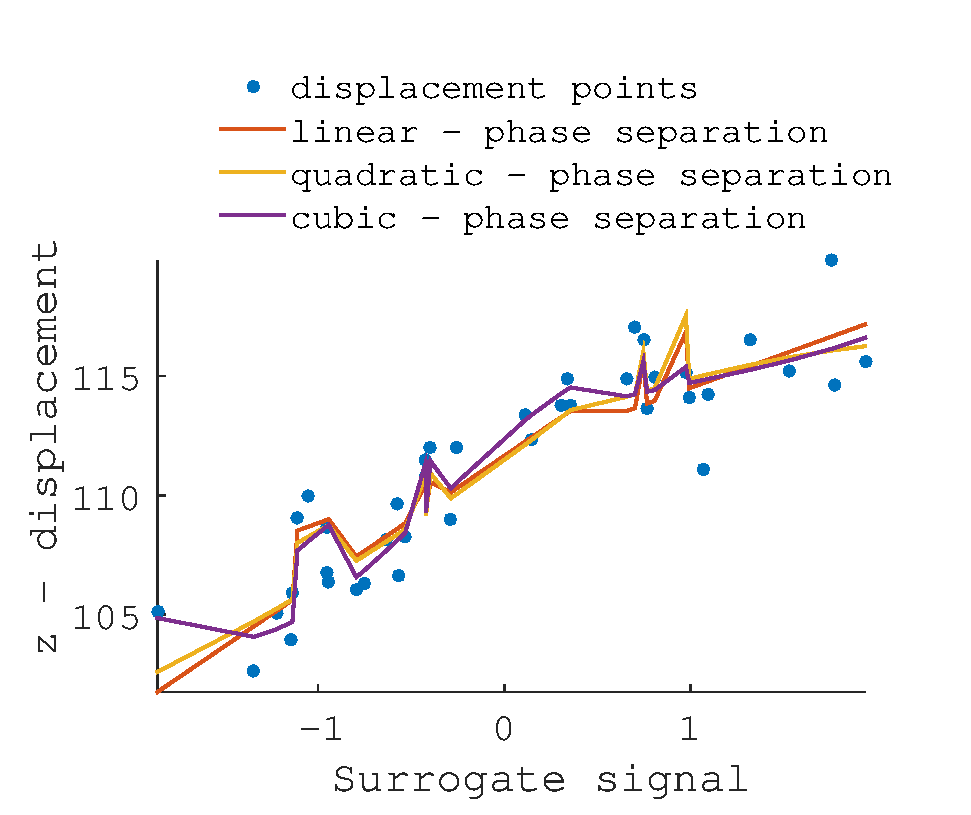
\includegraphics[width=\textwidth, trim=0 0 0 110,clip=true]{figures/task2/fit_round2_couch3.eps}
  \end{subfigure}
    ~ %add desired spacing between images, e. g. ~, \quad, \qquad, \hfill etc.
%     (or a blank line to force the subfigure onto a new line)
  \begin{subfigure}[b]{0.33\textwidth}
    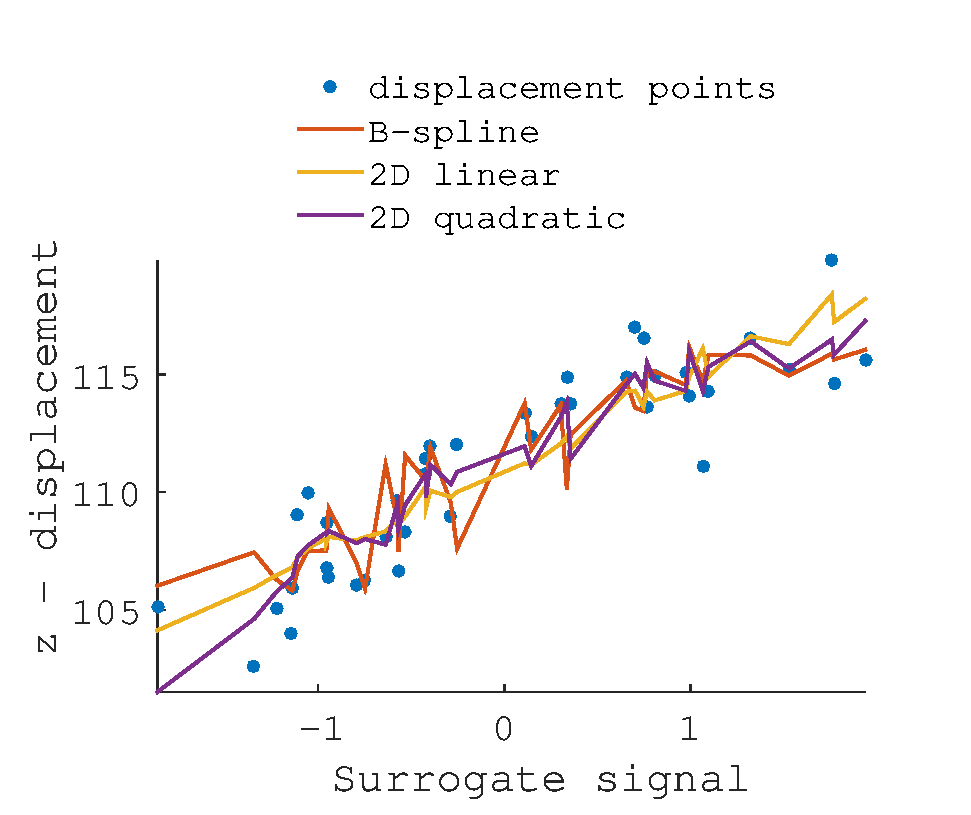
\includegraphics[width=\textwidth, trim=0 0 0 110,clip=true]{figures/task2/fit_round3_couch3.eps}
  \end{subfigure}
  (c) Fit for couch position 3, voxel (30,40,23,1,3)
  \vspace*{1em}
  
    \hspace*{-2em}
  \begin{subfigure}[b]{0.33\textwidth}
    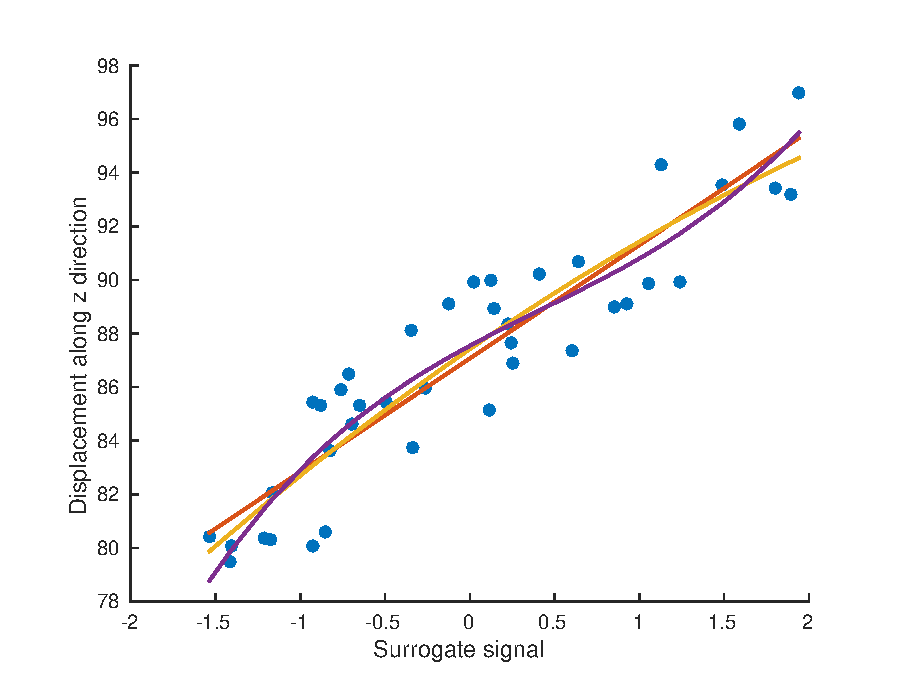
\includegraphics[width=\textwidth, trim=0 0 0 110,clip=true]{figures/task2/fit_round1_couch4.eps}
  \end{subfigure}%
    ~ %add desired spacing between images, e. g. ~, \quad, \qquad, \hfill etc.
%(or a blank line to force the subfigure onto a new line)
  \begin{subfigure}[b]{0.33\textwidth}
    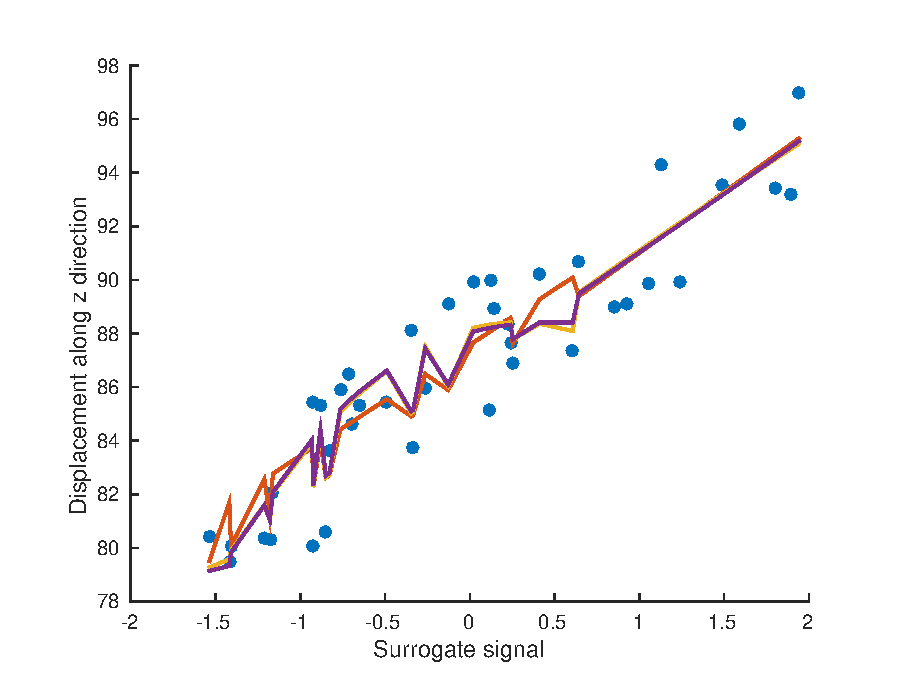
\includegraphics[width=\textwidth, trim=0 0 0 110,clip=true]{figures/task2/fit_round2_couch4.eps}
  \end{subfigure}
    ~ %add desired spacing between images, e. g. ~, \quad, \qquad, \hfill etc.
%     (or a blank line to force the subfigure onto a new line)
  \begin{subfigure}[b]{0.33\textwidth}
    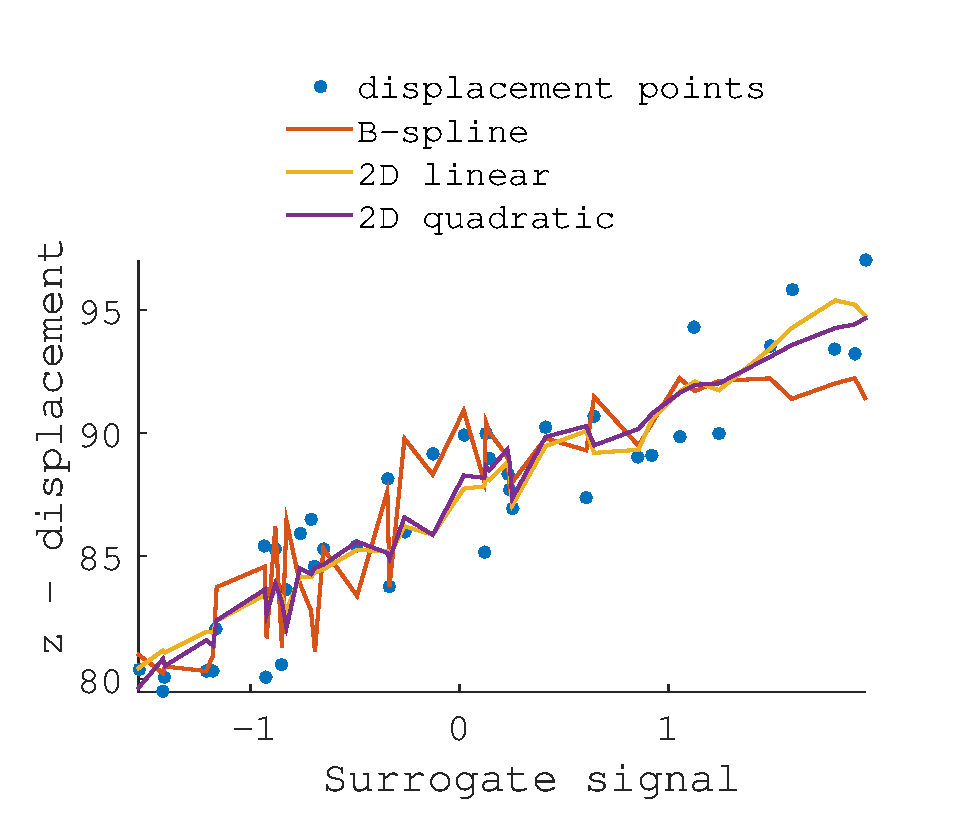
\includegraphics[width=\textwidth, trim=0 0 0 110,clip=true]{figures/task2/fit_round3_couch4.eps}
  \end{subfigure}
   (d) Fit for couch position 4, voxel (30,45,18,1,3)
  \vspace*{1em}

  
    \hspace*{-2em}
  \begin{subfigure}[b]{0.33\textwidth}
    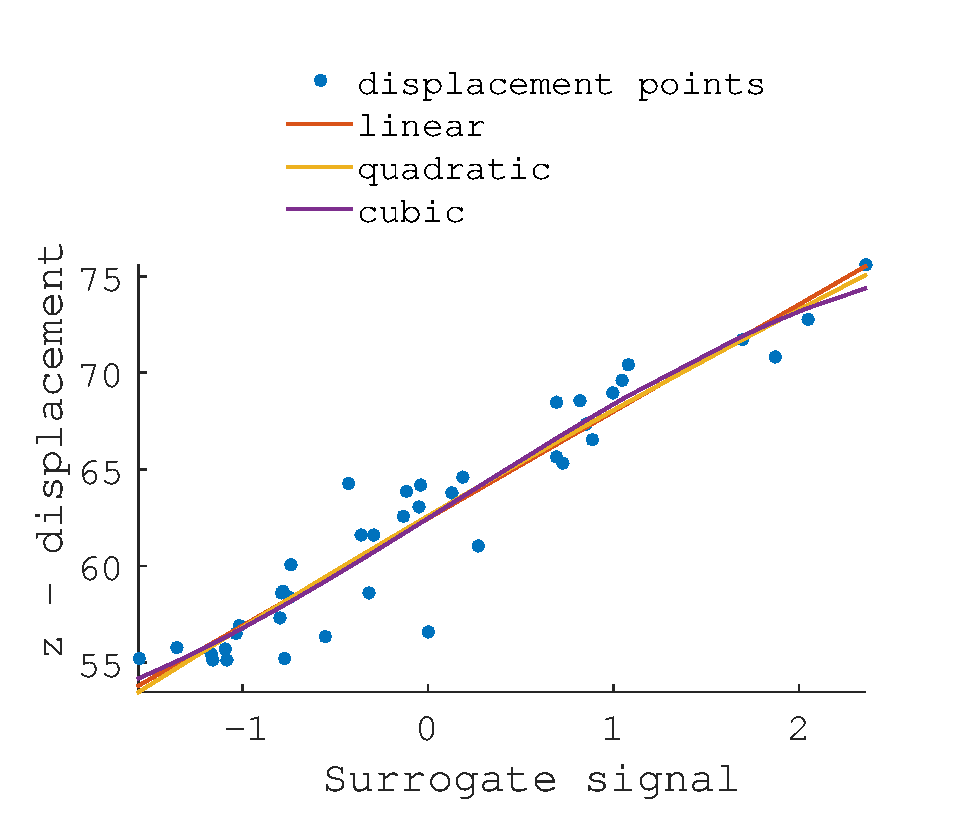
\includegraphics[width=\textwidth, trim=0 0 0 110,clip=true]{figures/task2/fit_round1_couch5.eps}
  \end{subfigure}%
    ~ %add desired spacing between images, e. g. ~, \quad, \qquad, \hfill etc.
%(or a blank line to force the subfigure onto a new line)
  \begin{subfigure}[b]{0.33\textwidth}
    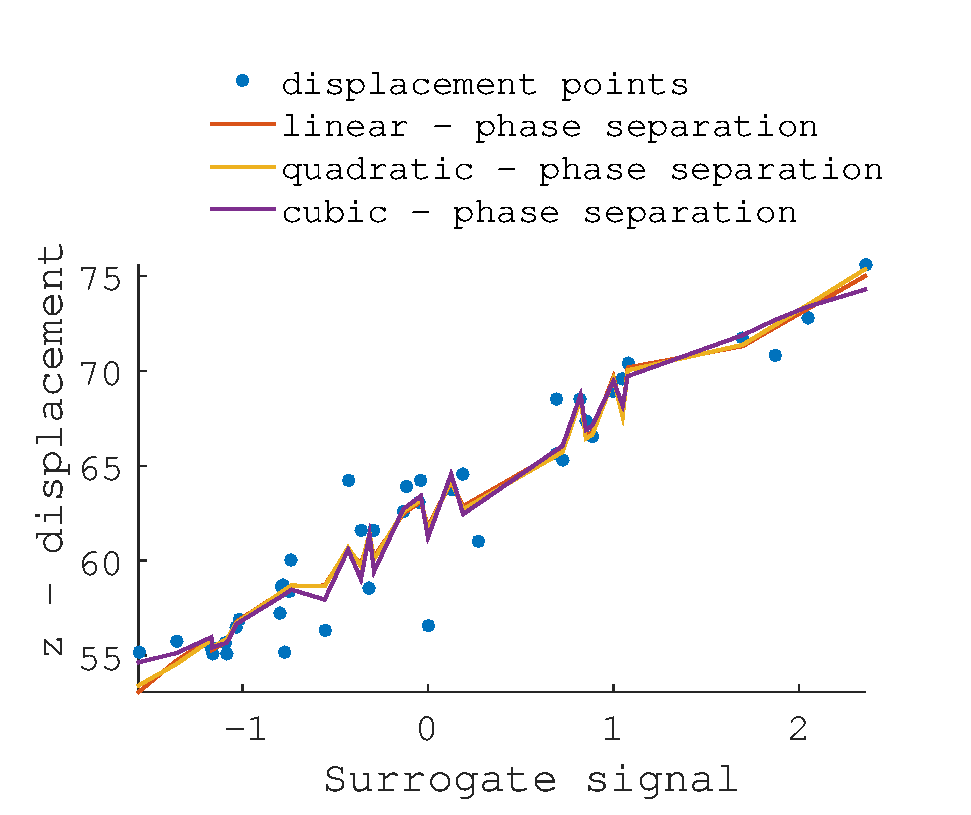
\includegraphics[width=\textwidth, trim=0 0 0 110,clip=true]{figures/task2/fit_round2_couch5.eps}
  \end{subfigure}
    ~ %add desired spacing between images, e. g. ~, \quad, \qquad, \hfill etc.
%     (or a blank line to force the subfigure onto a new line)
  \begin{subfigure}[b]{0.33\textwidth}
    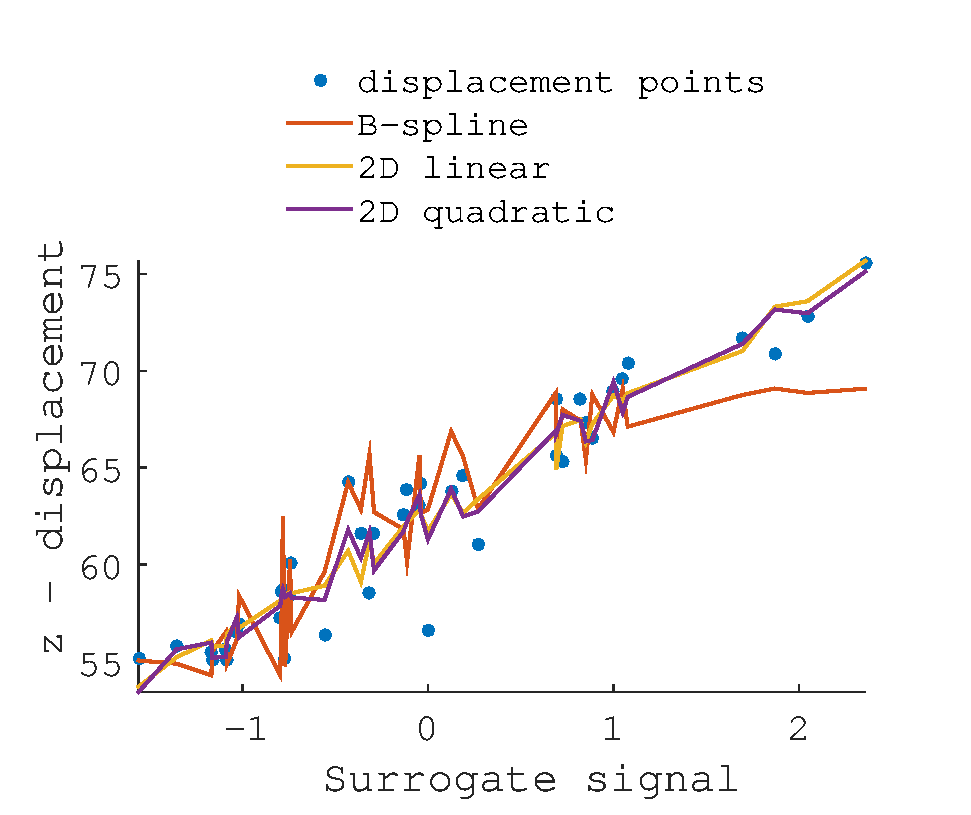
\includegraphics[width=\textwidth, trim=0 0 0 110,clip=true]{figures/task2/fit_round3_couch5.eps}
  \end{subfigure}
  (e) Fit for couch position 5, voxel (30,45,13,1,3)
  \vspace*{1em}

  
  \caption{Fit of 9 different models across 5 voxels each from a different couch position. The first column shows the fit for the three basic models: linear, quadratic and cubic. The second column shows the same models with phase separation, while the last column shows the fit for the B-spline, 2D linear and 2D quadratic models.}
  \label{fig:c2fit}
  
\end{figure}

I fit the models for one voxel by solving the GLM $D = SC$ where $D$ is the displacement along one direction, $S$ is the matrix of surrogate signals and $C$ are the coefficients. I chose to solve the GLM using the pseudo-inverse of $S^\top S$, giving $C = pinv(S^\top S)S^\top D$. I used the MATLAB function \texttt{pinv} because it can better handle singularities than the function \texttt{inv}. Figure \ref{fig:c2fit} shows the fit for 9 different models:
\begin{multicols}{3}
\begin{enumerate}
 \item linear
 \item quadratic
 \item cubic
 \item linear - phase separation
 \item quadratic - phase separation
 \item cubic - phase separation
 \item B-spline
 \item 2D linear
 \item 2D quadratic
\end{enumerate}
\end{multicols}

These models have been fit for all CP displacements using a fast (vectorised) method where all the CP displacements are flattened into a huge matrix. The fit is plotted in figure \ref{fig:c2fit} only for the given voxels for all the couch positions (one voxel/row with three groups of models for each plot).

The linear, quadratic and cubic models (plots in the column) give a reasonably good fit, especially for couch positions 4 and 5. The quadratic and cubic models don't differ much from the linear model, especially for voxels in couche positions 4 and 5. The phase separation models seem to fit outlier points better, but at the expense of extra parameters in the model. The B-spline and the 2D linear and quadratic models seem to fit the data best, but they run the risk of overfitting. The B-spline model seems to have a very oscilatory behaviour in the first few volumes, most evident in couch 2. In conclusion, all models fit these particular voxels well, and as we expected the more complex models give a better fit than the simpler models.

\subsection*{Task 4 - Evaluation of the motion models}

\subsubsection*{Visual Assessment}

Figure \ref{fig:c4visAss} shows the visual assessment for all the 9 models for couch 1, volume 1, slice 66. There is considerably more motion compared to the registration assessment in task 1. The results are quite good, with essentially no differences between the estimated defirmation across the models. The motion of the outer shape of the lung has been almost perfectly estimated, with tiny errors at the top corner of the right lung. More deformation errors are found at the vasculature of the right lung. We therefore conclude that all 9 models perform equally well.

\begin{figure}[H]
  \centering
  \hspace*{-2em}
  \begin{subfigure}[b]{0.33\textwidth}
    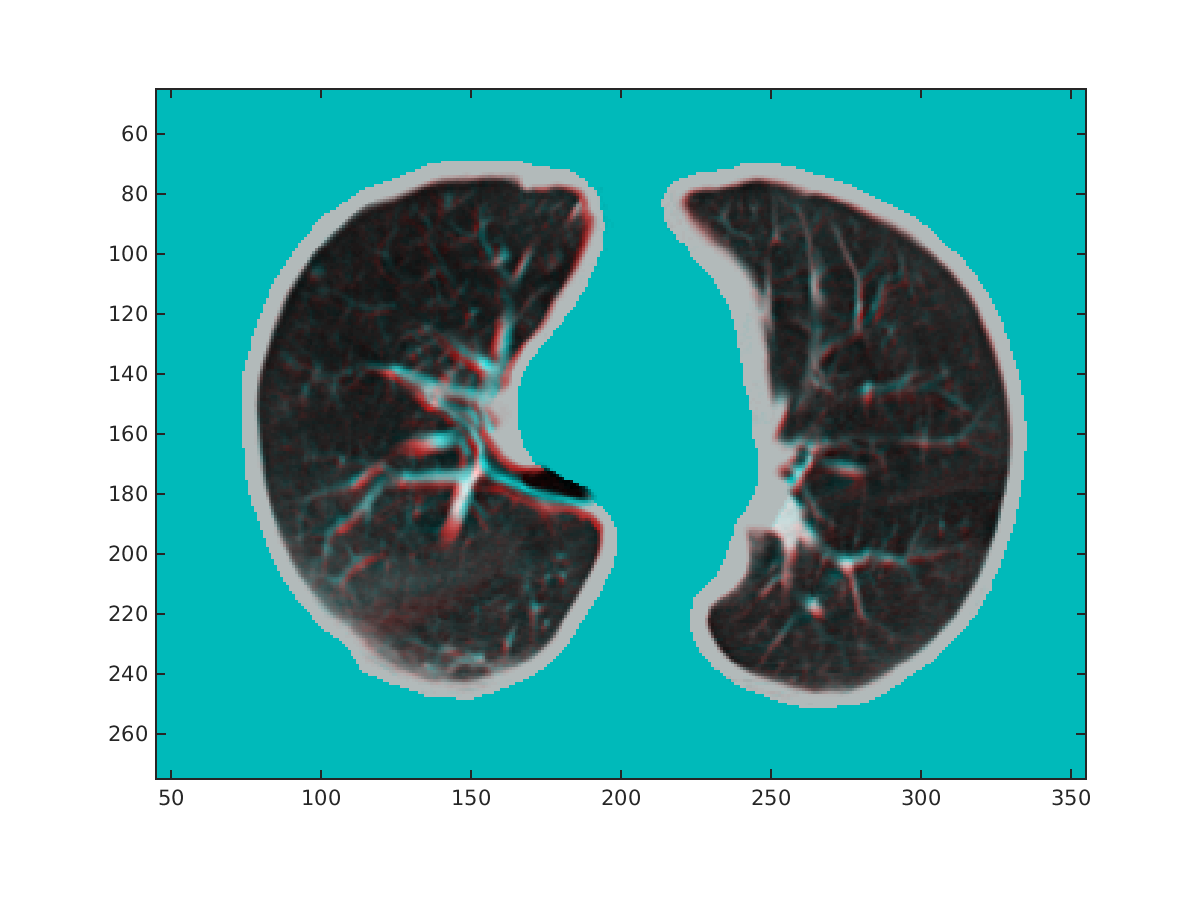
\includegraphics[width=\textwidth, trim=0 50 0 0,clip=true]{figures/task4/visAss_m1.png}
    \caption{Linear}
  \end{subfigure}%
  \begin{subfigure}[b]{0.33\textwidth}
    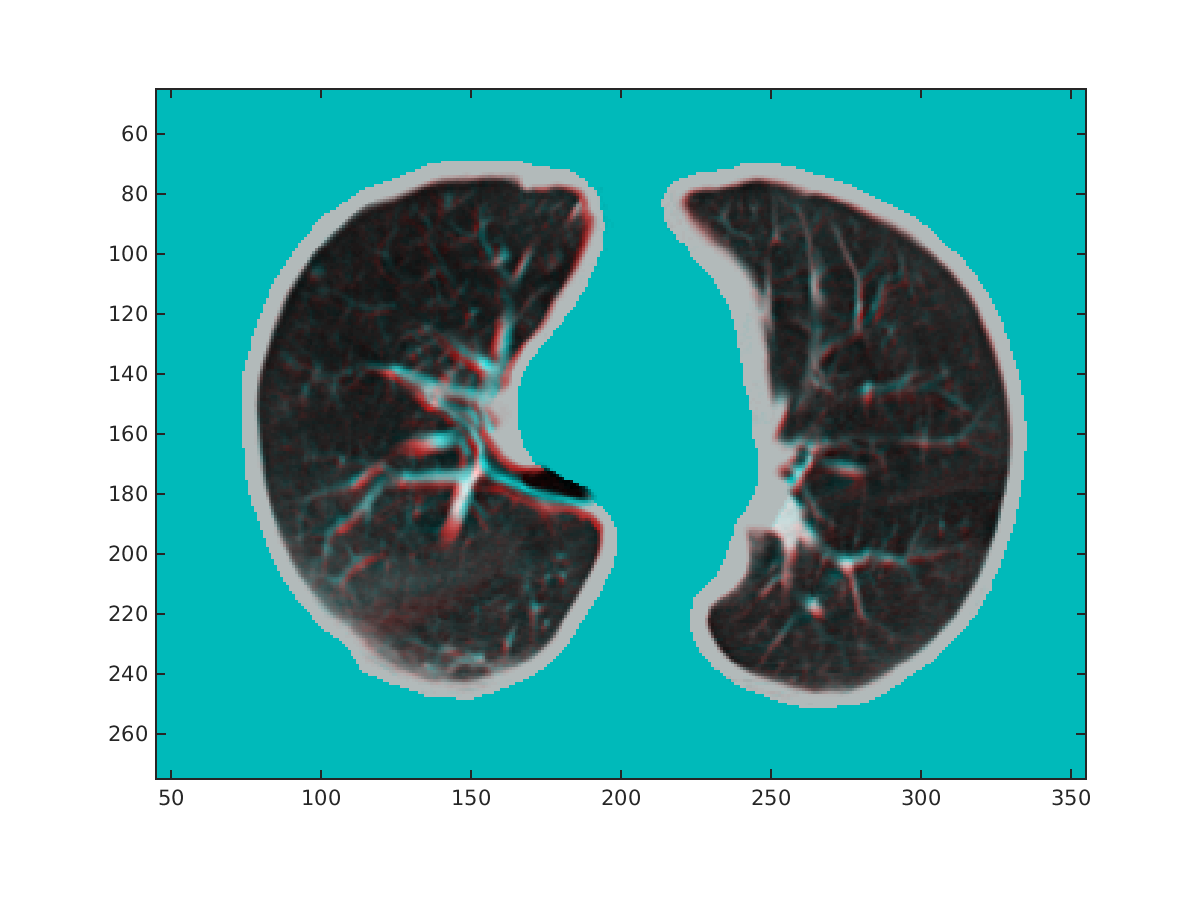
\includegraphics[width=\textwidth, trim=0 50 0 0,clip=true]{figures/task4/visAss_m1.png}
    \caption{Quadratic}
  \end{subfigure}
  \begin{subfigure}[b]{0.33\textwidth}
    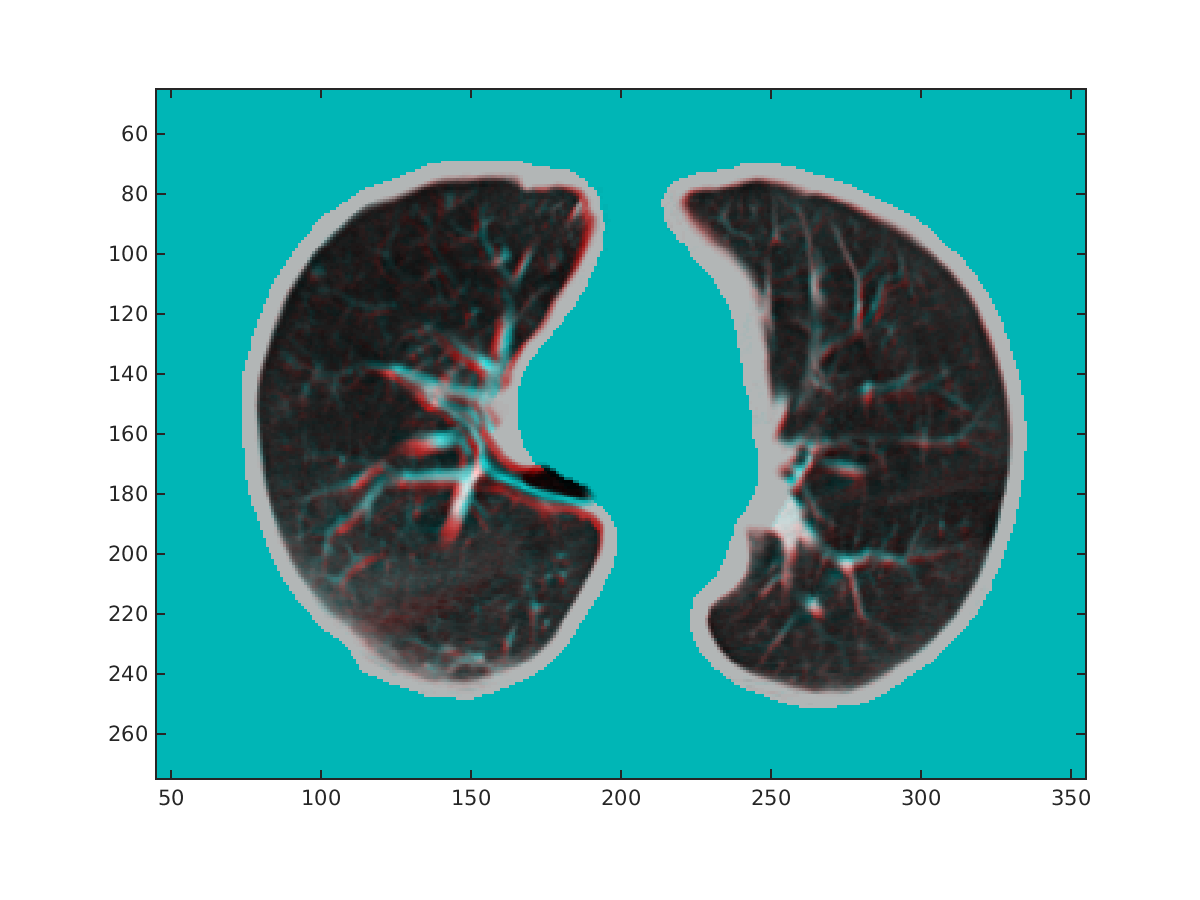
\includegraphics[width=\textwidth, trim=0 50 0 0,clip=true]{figures/task4/visAss_m3.png}
    \caption{Cubic}
  \end{subfigure}
  ~
  \hspace*{-2em}
  \begin{subfigure}[b]{0.33\textwidth}
    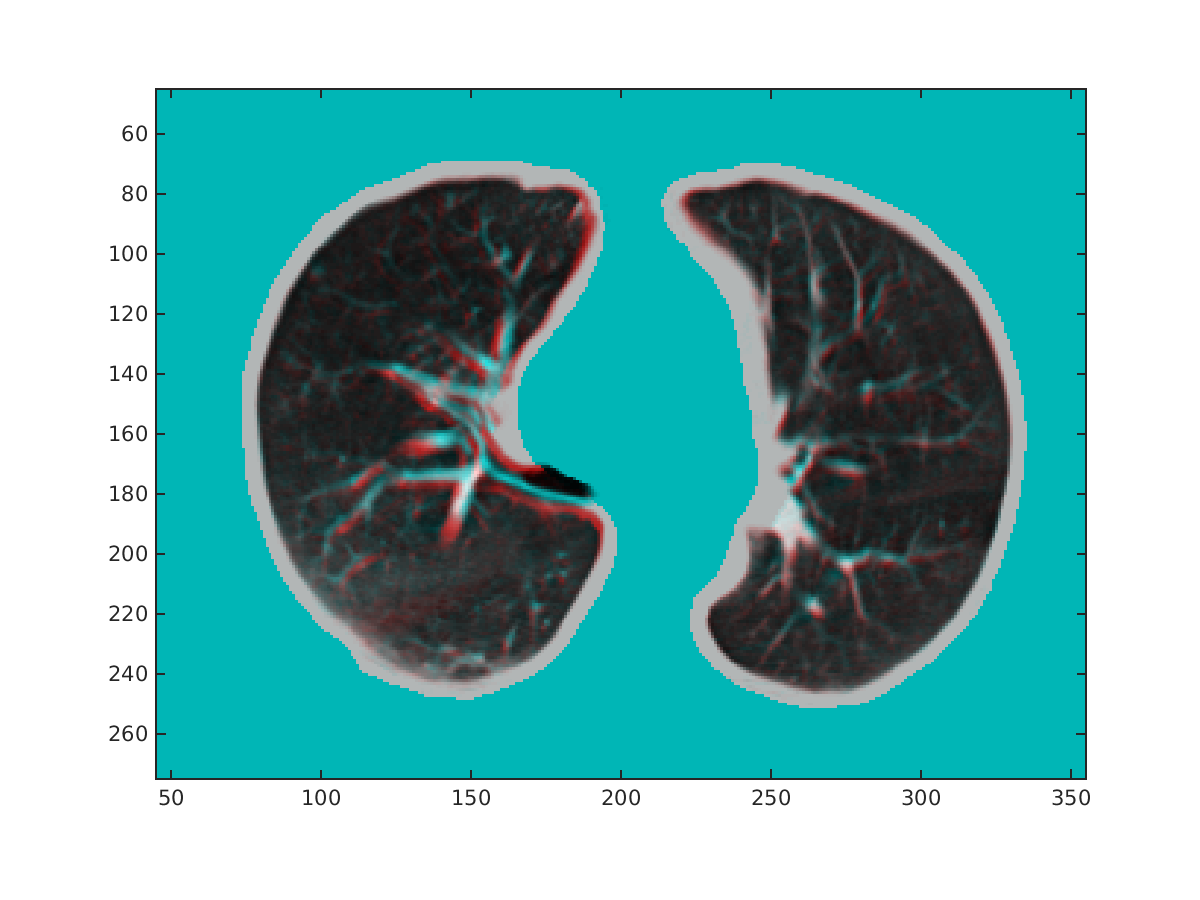
\includegraphics[width=\textwidth, trim=0 50 0 0,clip=true]{figures/task4/visAss_m4.png}
    \caption{Linear - Phase Separation}
  \end{subfigure}%
  \begin{subfigure}[b]{0.33\textwidth}
    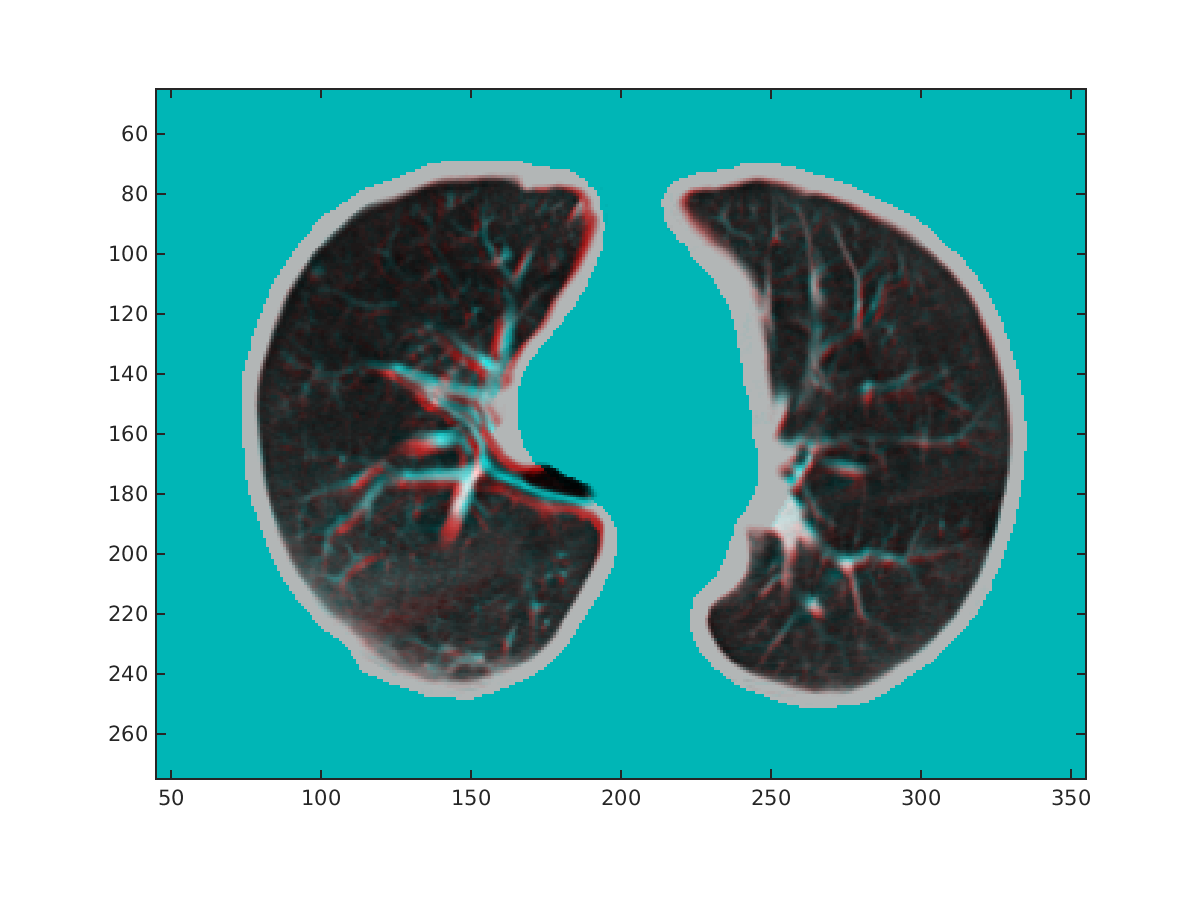
\includegraphics[width=\textwidth, trim=0 50 0 0,clip=true]{figures/task4/visAss_m5.png}
    \caption{Quadratic - Phase Separation}
  \end{subfigure}
  \begin{subfigure}[b]{0.33\textwidth}
    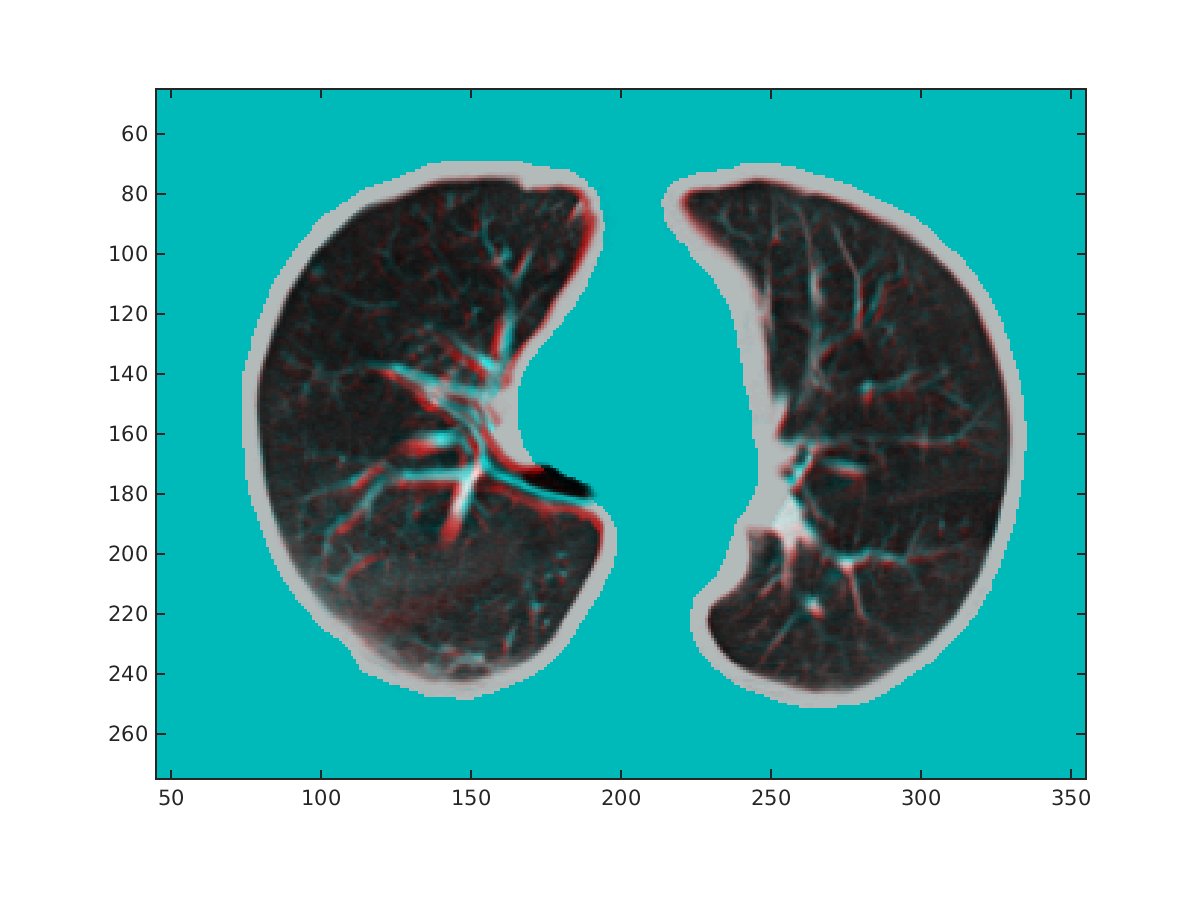
\includegraphics[width=\textwidth, trim=0 50 0 0,clip=true]{figures/task4/visAss_m6.png}
    \caption{Cubic - Phase Separation}
  \end{subfigure}
  ~
  \hspace*{-2em}
  \begin{subfigure}[b]{0.33\textwidth}
    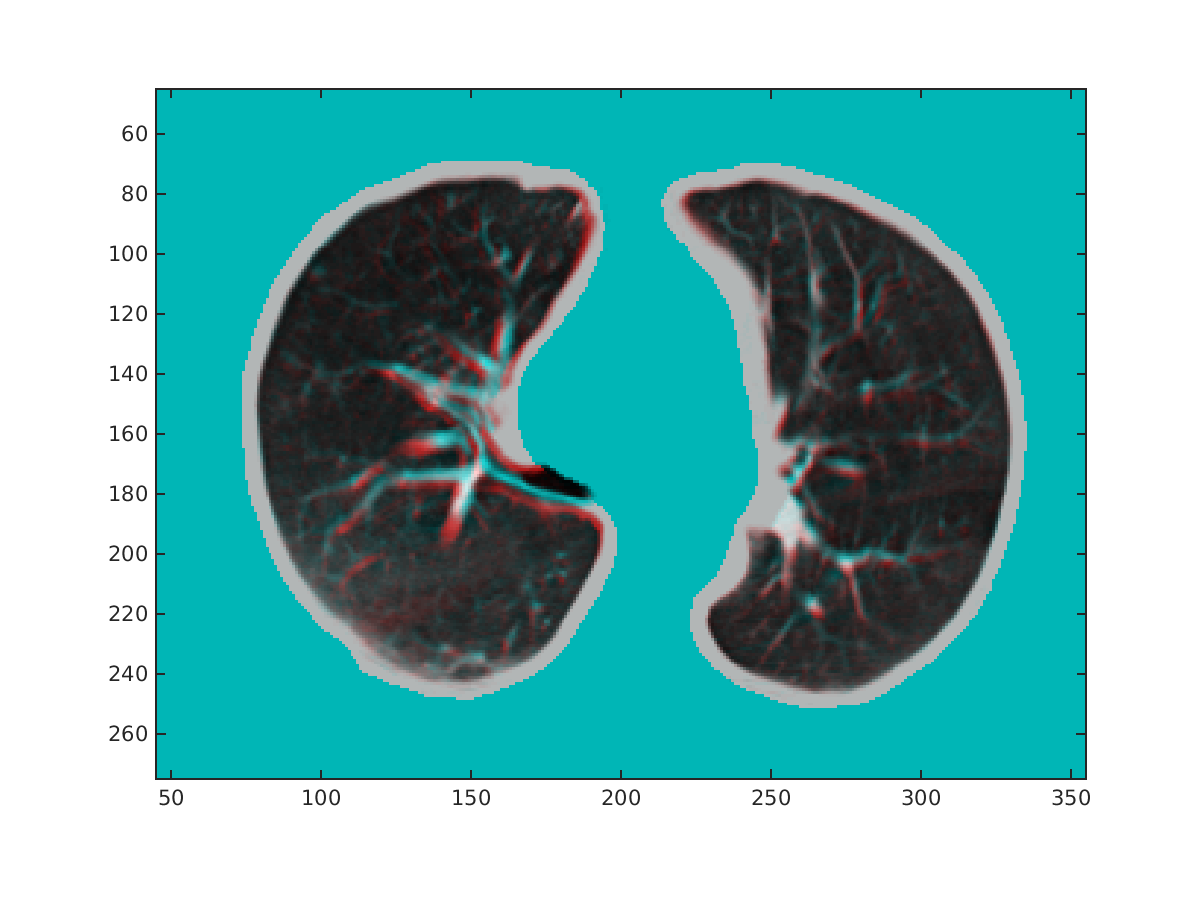
\includegraphics[width=\textwidth, trim=0 50 0 0,clip=true]{figures/task4/visAss_m7.png}
    \caption{B-spline}
  \end{subfigure}%
  \begin{subfigure}[b]{0.33\textwidth}
    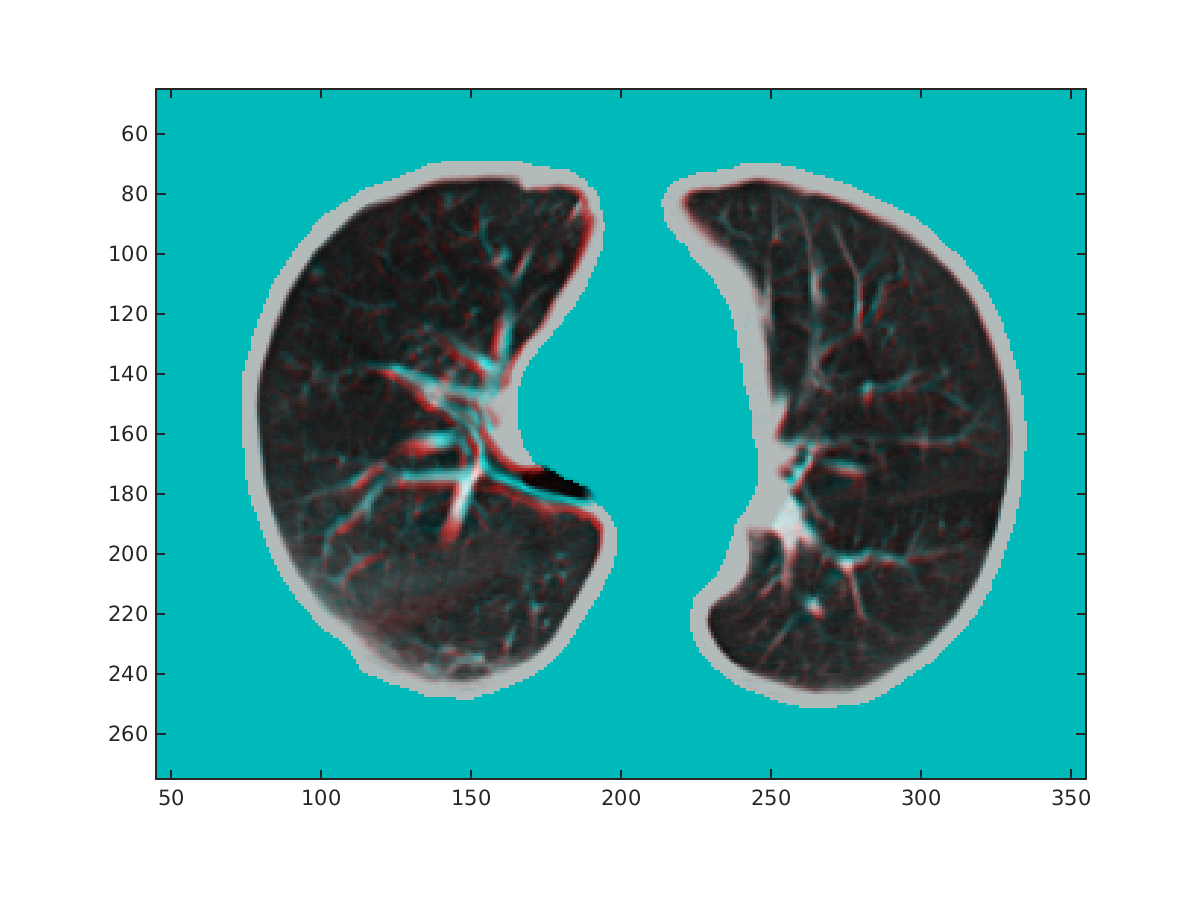
\includegraphics[width=\textwidth, trim=0 50 0 0,clip=true]{figures/task4/visAss_m8.png}
    \caption{Linear 2D}
  \end{subfigure}
  \begin{subfigure}[b]{0.33\textwidth}
    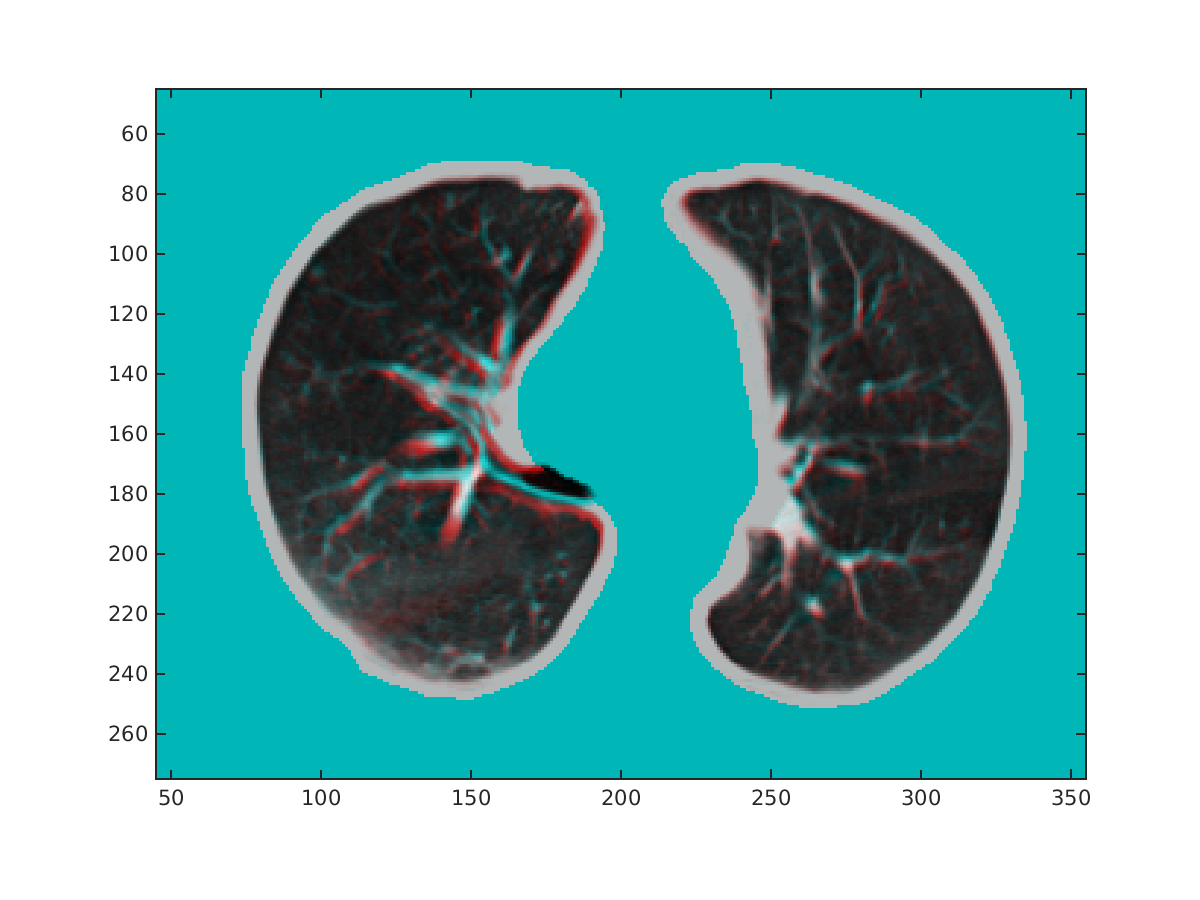
\includegraphics[width=\textwidth, trim=0 50 0 0,clip=true]{figures/task4/visAss_m9.png}
    \caption{Quadratic 2D}
  \end{subfigure}

    \caption{Visual assessment of the 9 deformation models using leave-one out cross-validation on couch 1, volume 1, slice 66. }
  \label{fig:c4visAss}
  
\end{figure}

\subsubsection*{Deformation Field Error}

Figure \ref{fig:c4defError} shows the deformation field error for the 10 Cine CT volumes across all 5 couch positions. The left column shows the mean error, while the right column shows the standard deviation. The ammount of motion varies slightly across the Cine CT scans but is usually less than 3mm. Similarly, standard deviation is usually below 1.2. The B-spline model seems to have larger error means and standard deviations especially in volumes from couch positions 4 and 5. The other models have similar errors across all couch positions.

\newcommand{\trimval}{140}
\newcommand{\trimvalleg}{140}

\begin{figure}[H]
  \centering
  \begin{subfigure}[b]{0.33\textwidth}
    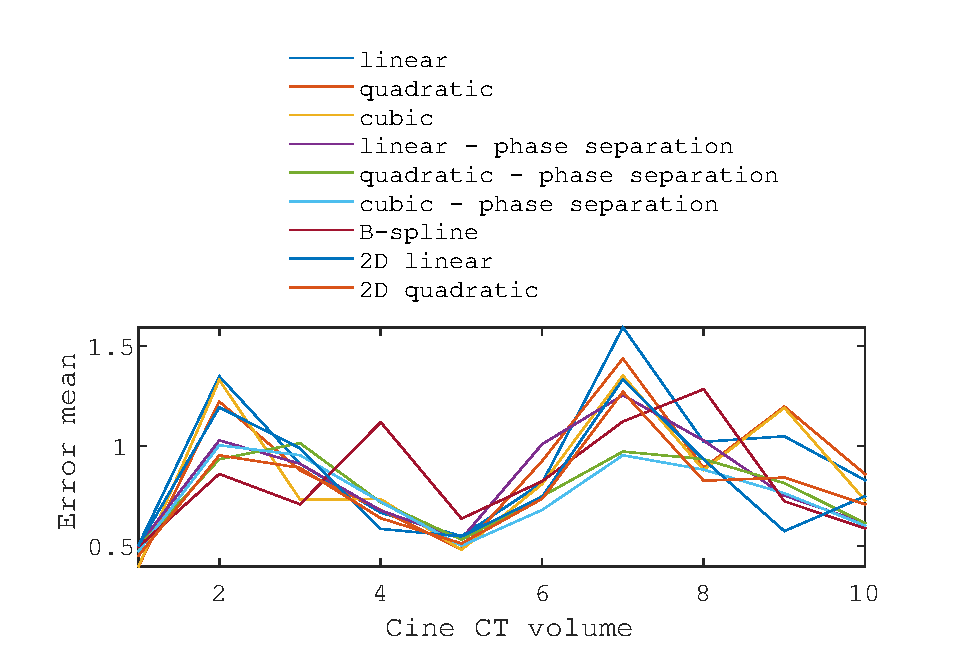
\includegraphics[width=\textwidth, trim=80 243 80 0,clip=true]{figures/task4/def_mean_error_couch1.eps}
  \end{subfigure}%
  \hspace{-3em}
  \begin{subfigure}[b]{0.33\textwidth}
    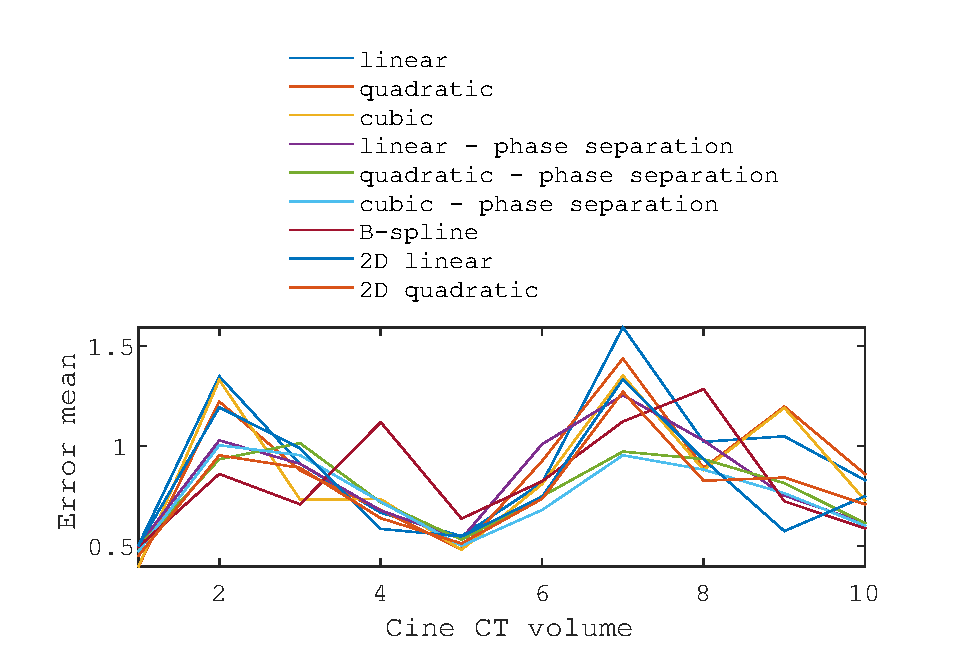
\includegraphics[width=\textwidth, trim=80 203 80 55,clip=true]{figures/task4/def_mean_error_couch1.eps}
  \end{subfigure}%
  \hspace{2em}
  \begin{subfigure}[b]{0.33\textwidth}
    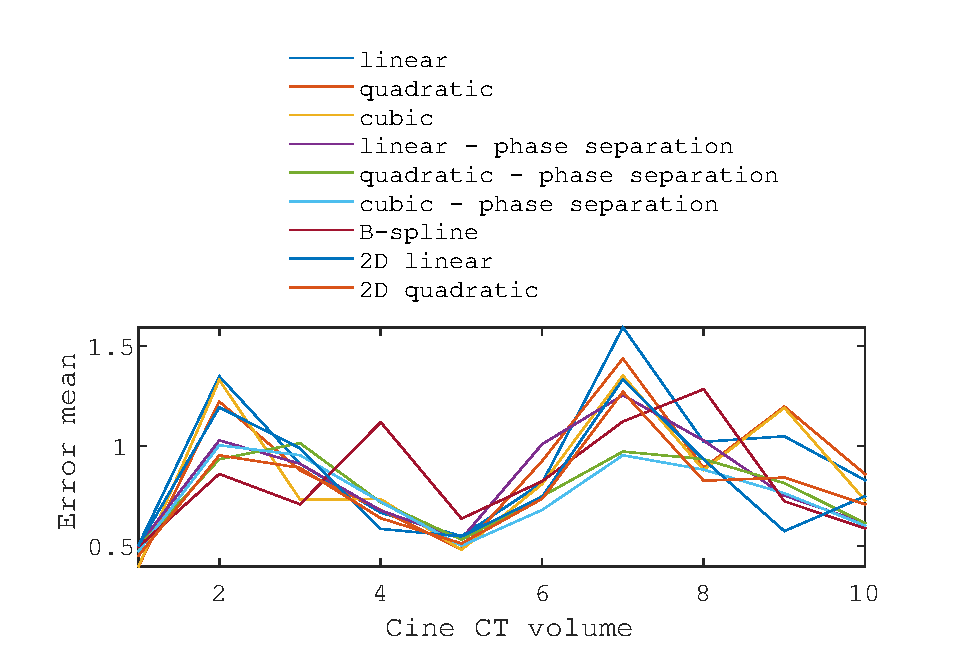
\includegraphics[width=\textwidth, trim=80 163 80 98,clip=true]{figures/task4/def_mean_error_couch1.eps}
  \end{subfigure}%
  
  \hspace*{-2em}
  \begin{subfigure}[b]{0.5\textwidth}
    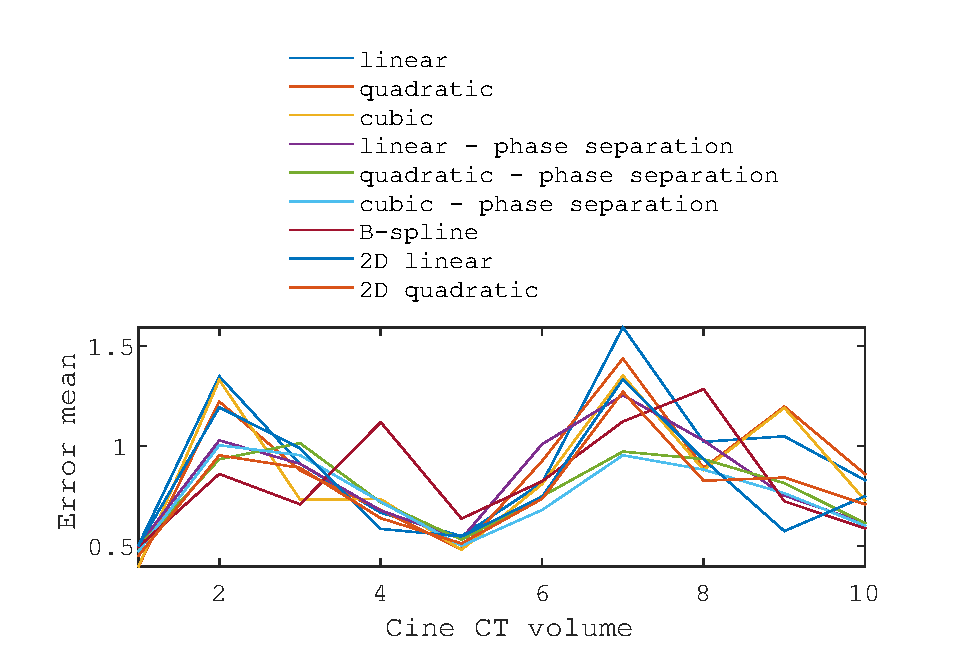
\includegraphics[width=\textwidth, trim=0 0 0 \trimval,clip=true]{figures/task4/def_mean_error_couch1.eps}
    \caption{Couch 1 - Mean Def. Error}
  \end{subfigure}%
  \begin{subfigure}[b]{0.5\textwidth}
    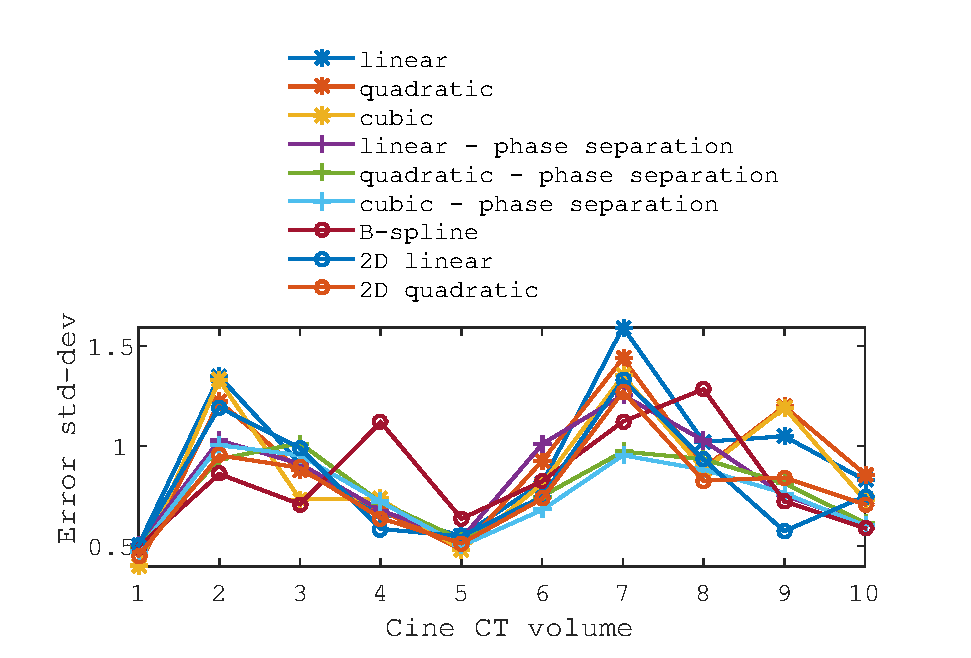
\includegraphics[width=\textwidth, trim=0 0 0 \trimval,clip=true]{figures/task4/def_stddev_error_couch1.eps}
    \caption{Couch 1 - Std. Dev. of Def. Error}
  \end{subfigure}
  ~
    \hspace*{-2em}
  \begin{subfigure}[b]{0.5\textwidth}
    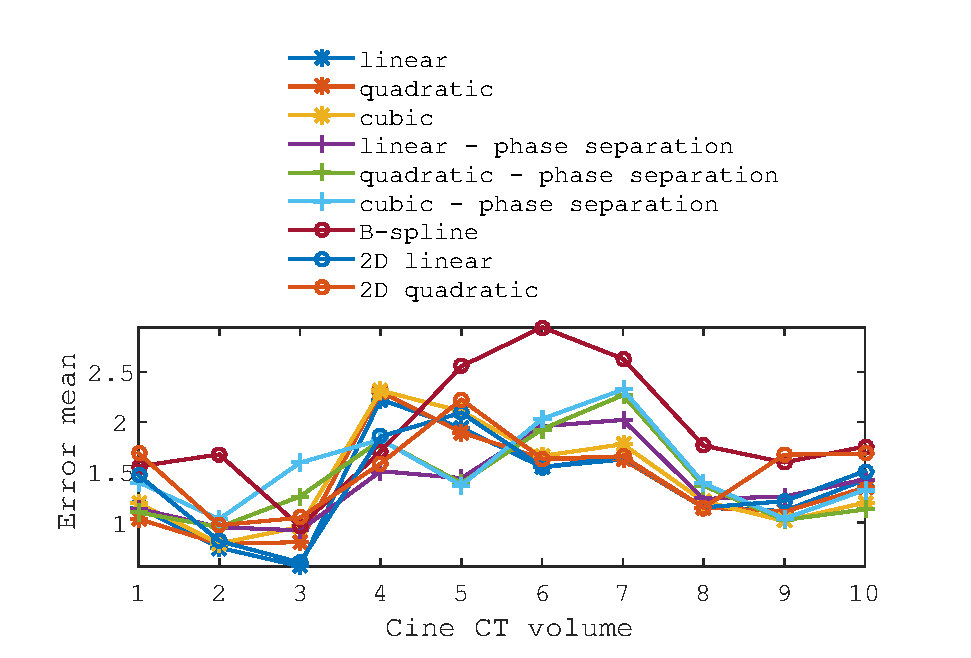
\includegraphics[width=\textwidth, trim=0 0 0 \trimval,clip=true]{figures/task4/def_mean_error_couch2.eps}
    \caption{Couch 2 - Mean Def. Error}
  \end{subfigure}%
  \begin{subfigure}[b]{0.5\textwidth}
    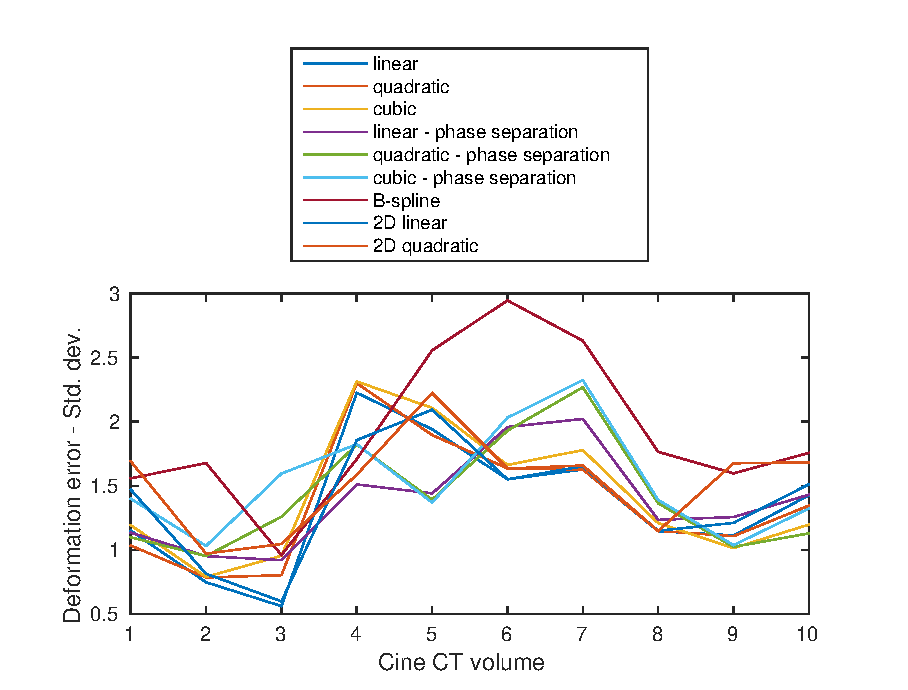
\includegraphics[width=\textwidth, trim=0 0 0 \trimval,clip=true]{figures/task4/def_stddev_error_couch2.eps}
    \caption{Couch 2 - Std. Dev. of Def. Error}
  \end{subfigure}
  ~
    \hspace*{-2em}
  \begin{subfigure}[b]{0.5\textwidth}
    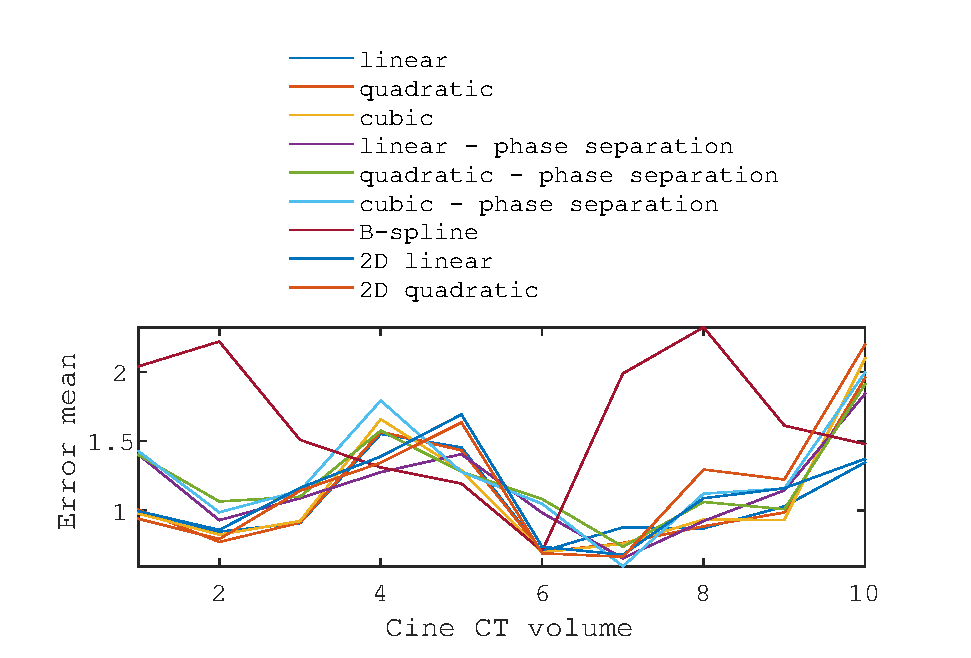
\includegraphics[width=\textwidth, trim=0 0 0 \trimval,clip=true]{figures/task4/def_mean_error_couch3.eps}
    \caption{Couch 3 - Mean Def. Error}
  \end{subfigure}%
  \begin{subfigure}[b]{0.5\textwidth}
    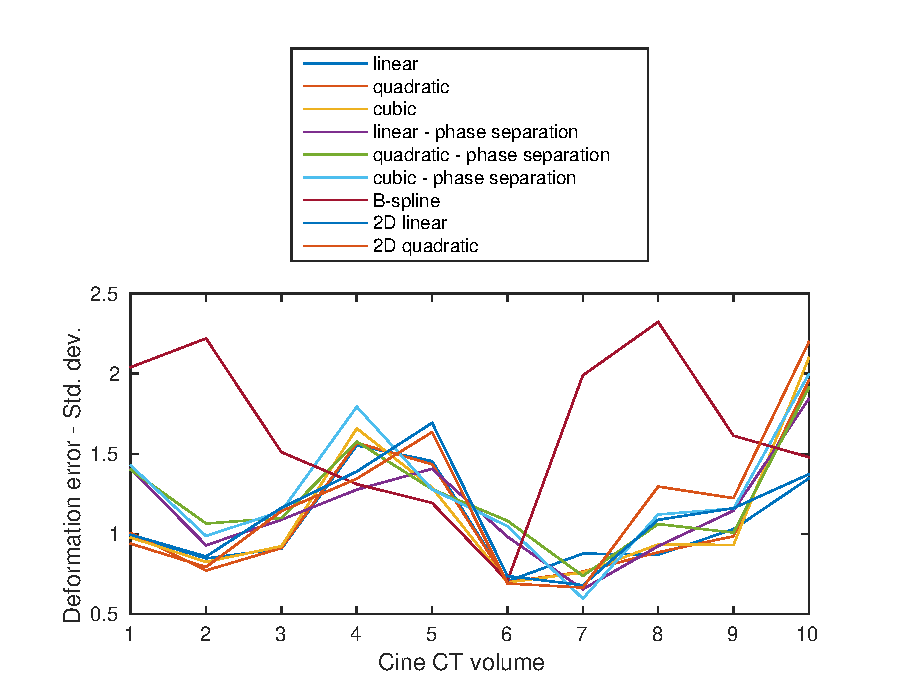
\includegraphics[width=\textwidth, trim=0 0 0 \trimval,clip=true]{figures/task4/def_stddev_error_couch3.eps}
    \caption{Couch 3 - Std. Dev. of Def. Error}
  \end{subfigure}
  ~
    \hspace*{-2em}
  \begin{subfigure}[b]{0.5\textwidth}
    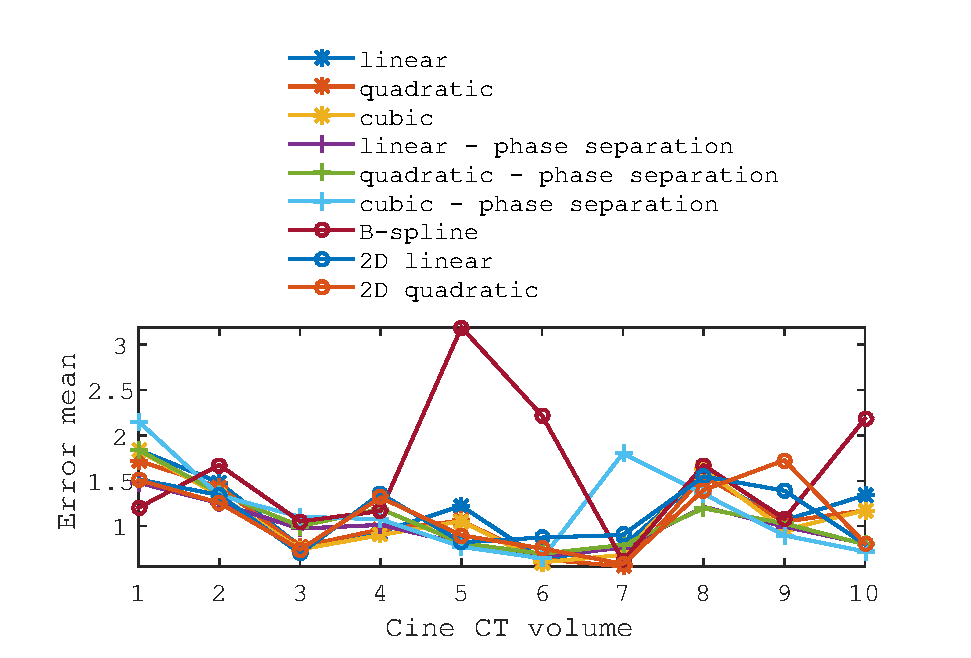
\includegraphics[width=\textwidth, trim=0 0 0 \trimval,clip=true]{figures/task4/def_mean_error_couch4.eps}
    \caption{Couch 4 - Mean Def. Error}
  \end{subfigure}%
  \begin{subfigure}[b]{0.5\textwidth}
    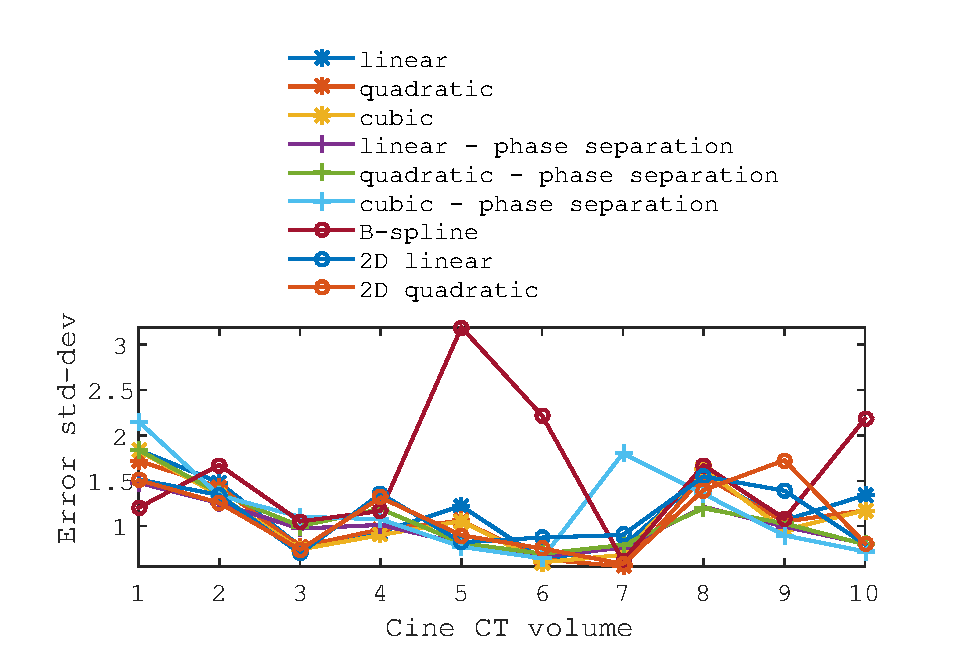
\includegraphics[width=\textwidth, trim=0 0 0 \trimval,clip=true]{figures/task4/def_stddev_error_couch4.eps}
    \caption{Couch 4 - Std. Dev. of Def. Error}
  \end{subfigure}
  ~
    \hspace*{-2em}
  \begin{subfigure}[b]{0.5\textwidth}
    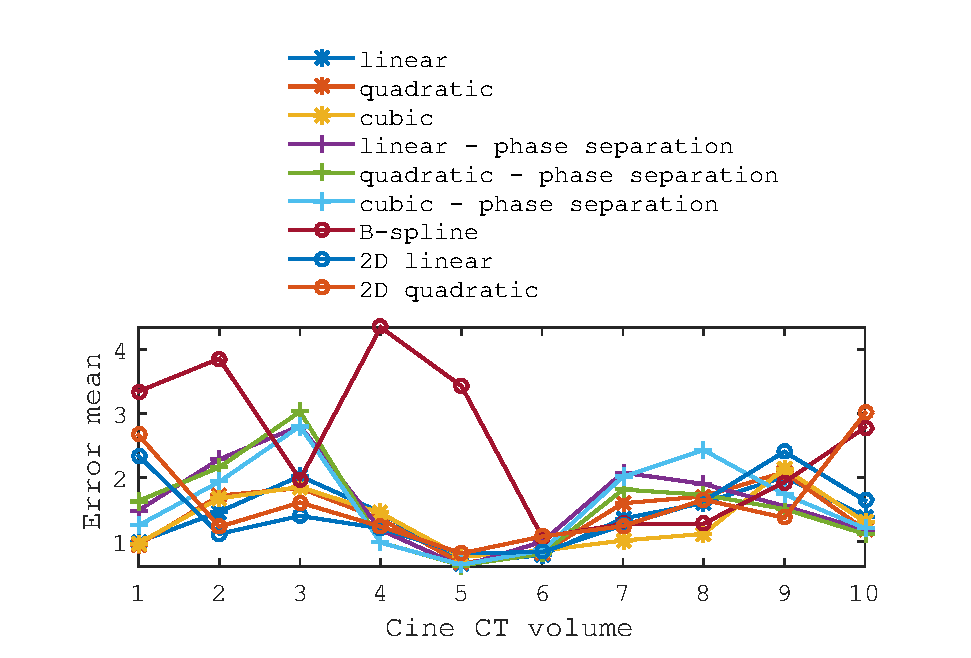
\includegraphics[width=\textwidth, trim=0 0 0 \trimval,clip=true]{figures/task4/def_mean_error_couch5.eps}
    \caption{Couch 5 - Mean Def. Error}
  \end{subfigure}%
  \begin{subfigure}[b]{0.5\textwidth}
    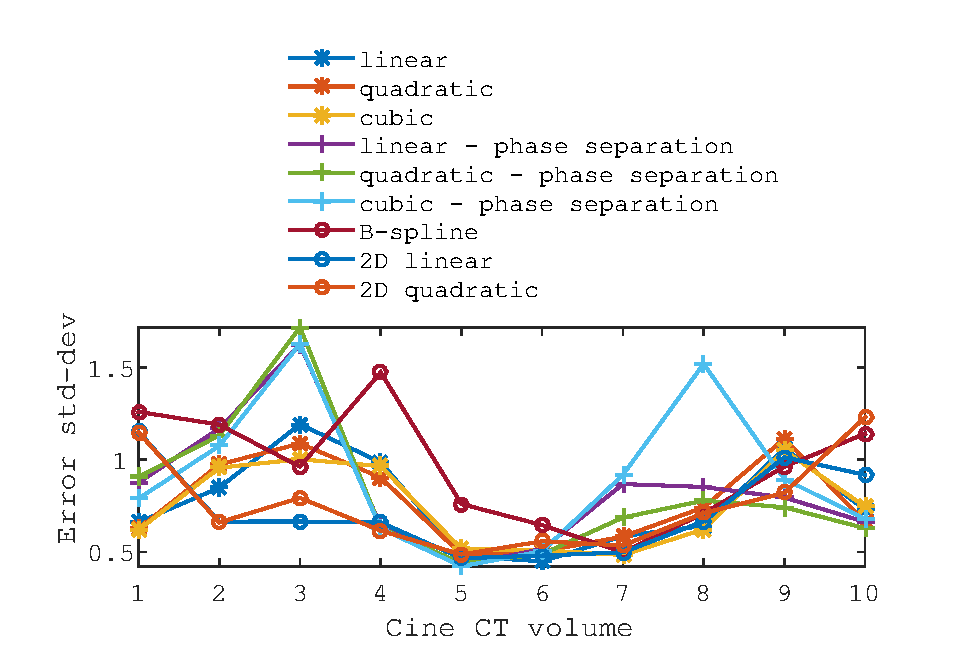
\includegraphics[width=\textwidth, trim=0 0 0 \trimval,clip=true]{figures/task4/def_stddev_error_couch5.eps}
    \caption{Couch 5 - Std. Dev. of Def. Error}
  \end{subfigure}
  ~
  \caption{Deformation Error mean and standard deviation for all 5 couch positions, 10 Cine CT volumes and 9 models.}
  \label{fig:c4defError}
  
\end{figure}

\subsubsection*{Landmark Error}

Figure \ref{fig:c4landError} shows the landmark errors for all the 9 models across the 5 couch positions, this time using all 40 Cine CT volumes. Moreover, the landmark error using the original registration is also plotted in black. The landmark error is usually between 1 and 4mm. All models perform equally good, with no clear winner from the plots. In particular, the cubic - phase separation model seems to have a spike in landmark error at couch position 2, volume 24, which might be due to overfitting. 

\begin{figure}[H]
%   \centering
  \begin{subfigure}[b]{0.5\textwidth}
    \includegraphics[width=\textwidth, trim=0 0 0 0,clip=true]{figures/task4/landmark_error_couch1.eps}
    \caption{Couch 1}
  \end{subfigure}%
  \begin{subfigure}[b]{0.32\textwidth}
    \includegraphics[width=\textwidth, trim=410 0 0 0,clip=true]{figures/task4/landmark_error_legend.eps}\\
  \end{subfigure}%
  
  \begin{subfigure}[b]{0.5\textwidth}
    \includegraphics[width=\textwidth, trim=0 0 0 0,clip=true]{figures/task4/landmark_error_couch2.eps}
    \caption{Couch 2}
  \end{subfigure}%
  \begin{subfigure}[b]{0.5\textwidth}
    \includegraphics[width=\textwidth, trim=0 0 0 0,clip=true]{figures/task4/landmark_error_couch3.eps}
    \caption{Couch 3}
  \end{subfigure}%
   
  \begin{subfigure}[b]{0.5\textwidth}
    \includegraphics[width=\textwidth, trim=0 0 0 0,clip=true]{figures/task4/landmark_error_couch4.eps}
    \caption{Couch 4}
  \end{subfigure}%
  \begin{subfigure}[b]{0.5\textwidth}
    \includegraphics[width=\textwidth, trim=0 0 0 0,clip=true]{figures/task4/landmark_error_couch5.eps}
    \caption{Couch 5}
  \end{subfigure}%
  
  \caption{Landmark error for all 5 couch positions, 40 Cine CT volumes and 9 models.}
  \label{fig:c4landError}
  
\end{figure}

\subsubsection*{Model Ranking}


\subsection*{Task 5 - Parameter uncertainty}

\begin{figure}[H]
   \centering
    \begin{subfigure}[b]{0.4\textwidth}
    \includegraphics[width=\textwidth, trim=0 15 0 0,clip=true]{figures/task5/uncert_legend.eps}
%     \caption{Parameter 2}
  \end{subfigure}%

  \begin{subfigure}[b]{0.5\textwidth}
    \includegraphics[width=\textwidth, trim=0 0 0 0,clip=true]{figures/task5/uncert_model1_param1.eps}
    \caption{Parameter 1}
  \end{subfigure}%
  \begin{subfigure}[b]{0.5\textwidth}
    \includegraphics[width=\textwidth, trim=0 0 0 0,clip=true]{figures/task5/uncert_model1_param2.eps}
    \caption{Parameter 2}
  \end{subfigure}%
  
  \caption{Parameter uncertainty for the linear model.}
  \label{fig:c5uncertM1}
  
\end{figure}

\begin{figure}[H]
   \centering
     \begin{subfigure}[b]{0.5\textwidth}
    \includegraphics[width=\textwidth, trim=0 0 0 0,clip=true]{figures/task5/uncert_model2_param1.eps}
    \caption{Parameter 1}
  \end{subfigure}%
    \begin{subfigure}[b]{0.5\textwidth}
    \includegraphics[width=0.8\textwidth, trim=0 15 0 0,clip=true]{figures/task5/uncert_legend.eps}\\\\\\
%     \caption{Parameter 2}
  \end{subfigure}%
  
  \begin{subfigure}[b]{0.5\textwidth}
    \includegraphics[width=\textwidth, trim=0 0 0 0,clip=true]{figures/task5/uncert_model2_param2.eps}
    \caption{Parameter 2}
  \end{subfigure}%
  \begin{subfigure}[b]{0.5\textwidth}
    \includegraphics[width=\textwidth, trim=0 0 0 0,clip=true]{figures/task5/uncert_model2_param2.eps}
    \caption{Parameter 3}
  \end{subfigure}%
  
  \caption{Parameter uncertainty for the quadratic model.}
  \label{fig:c5uncertM1}
  
\end{figure}

\begin{figure}[H]
   \centering
    \begin{subfigure}[b]{0.5\textwidth}
    \includegraphics[width=0.8\textwidth, trim=0 15 0 0,clip=true]{figures/task5/uncert_legend.eps}
  \end{subfigure}%
  
  \begin{subfigure}[b]{0.5\textwidth}
    \includegraphics[width=\textwidth, trim=0 0 0 0,clip=true]{figures/task5/uncert_model3_param1.eps}
    \caption{Parameter 1}
  \end{subfigure}%
  \begin{subfigure}[b]{0.5\textwidth}
    \includegraphics[width=\textwidth, trim=0 0 0 0,clip=true]{figures/task5/uncert_model3_param2.eps}
    \caption{Parameter 2}
  \end{subfigure}%
  
  \begin{subfigure}[b]{0.5\textwidth}
    \includegraphics[width=\textwidth, trim=0 0 0 0,clip=true]{figures/task5/uncert_model3_param3.eps}
    \caption{Parameter 2}
  \end{subfigure}%
  \begin{subfigure}[b]{0.5\textwidth}
    \includegraphics[width=\textwidth, trim=0 0 0 0,clip=true]{figures/task5/uncert_model3_param4.eps}
    \caption{Parameter 3}
  \end{subfigure}%
  
  \caption{Parameter uncertainty for the cubic model.}
  \label{fig:c5uncertM1}
  
\end{figure}

\subsection*{Advanced tasks}







\end{document}





















